% arara: pdflatex
% arara: bibtex 
% arara: pdflatex 
% arara: pdflatex 
\documentclass[smallextended,natbib]{svjour3} %
\RequirePackage{fix-cm}
\usepackage[T1]{fontenc}
\usepackage[utf8]{inputenc}

%\usepackage{showframe}

\usepackage{textcomp} 
\usepackage{setspace}

\usepackage{caption} 
\usepackage{subcaption} 
\usepackage{afterpage} 

\usepackage{slantsc}
\usepackage{pifont}
\newcommand{\xmark}{\ding{54}}%
\newcommand{\ymark}{\ding{56}}%
\newcommand{\sunmark}{\ding{106}}%
\newcommand{\handmark}{\ding{43}}%

% \usepackage{lineno}
% \usepackage{pagecolor}
% \pagecolor{yellow!10!orange!5}

\usepackage[framemethod=tikz]{mdframed}
\mdfsetup{
skipabove=\baselineskip,
skipbelow=\baselineskip,
innertopmargin=3pt,
innerbottommargin=8pt,
apptotikzsetting={\tikzset{mdfbackground/.append style={fill=red,fill opacity=0}}}
}



%% \usepackage{fontspec}
%% \newfontfamily{\tam}[Script=Tamil]{Lohit Tamil}
%% \defaultfontfeatures{Scale=MatchLowercase}

\usepackage{eurosym}

\usepackage{url}
%\usepackage{apacite}            % APA style citations
%\usepackage{apacdoc}

\let\oldcite\cite
\let\cite\citep
\let\citeA\oldcite
\let\citeNP\oldcite
\let\citeyear\citeyearpar
%\let\citeyear\cite

\usepackage{amsmath,amssymb}	% math structures and symbols
\usepackage{graphicx}		% including of graphics files in various formats
\usepackage{amsfonts}

\let\proof\relax
\let\endproof\relax 
\usepackage{amsthm}

\newtheorem*{ndef}{Definition of serendipity}

\newtheoremstyle{named}{.2\topsep}{}{\itshape}{}{\bfseries}{.}{}{}
\theoremstyle{named}


\usepackage{dialogue}
\usepackage{placeins}
\usepackage{tikz}
\usepackage{onimage}
\usetikzlibrary{positioning,backgrounds,fit,arrows,arrows.meta,shapes,shadows}
\usetikzlibrary{shapes.multipart}
\usepackage{wrapfig}
\usepackage{enumitem}
\usepackage{framed}

% \hypersetup{hidelinks}

\usepackage[xspace,mla]{ellipsis}

\definecolor{myyellow}{RGB}{242,226,149}
\definecolor{mygreen}{RGB}{144,238,144}
\definecolor{mypink}{RGB}{255,182,193}
\definecolor{myorange}{RGB}{255,165,0}
\definecolor{myblue}{RGB}{0,204,204}

\usepackage{xparse}
\NewDocumentCommand\StickyNote{O{4cm}mmO{4cm}}{%
\begin{tikzpicture}
\node[
drop shadow={
  shadow xshift=2pt,
  shadow yshift=-4pt
},
inner xsep=7pt,
fill=#2,
xslant=-0.05,
yslant=0.05,
inner ysep=10pt
] {\parbox[t][#1][c]{#4}{#3}};
\end{tikzpicture}%
}

%\urldef{\mailsa}\path|{j.corneli,s.colton}@gold.ac.uk|
%\urldef{\mailsb}\path|a.pease@dundee.co.uk|

%% \newcommand{\keywords}[1]{\par\addvspace\baselineskip
%% \noindent\keywordname\enspace\ignorespaces#1}

\usepackage{array,booktabs}
\newcommand{\tcap}[1]{
\begin{minipage}{.7in}
{\centering #1 \par}
\end{minipage}
}

\newcommand{\inlineitem}[1]{%
\begingroup%
\setlength\itemindent{-1em}%
\item[]%
\begin{minipage}{.96\textwidth}%
#1%
\end{minipage}%
\endgroup
}


\usepackage[ocgcolorlinks,citecolor=blue]{hyperref}

% Patch for just citing years are cited
\usepackage{etoolbox}

\makeatletter

% Patch case where name and year are separated by aysep
\patchcmd{\NAT@citex}
  {\@citea\NAT@hyper@{%
     \NAT@nmfmt{\NAT@nm}%
     \hyper@natlinkbreak{\NAT@aysep\NAT@spacechar}{\@citeb\@extra@b@citeb}%
     \NAT@date}}
  {\@citea\NAT@nmfmt{\NAT@nm}%
   \NAT@aysep\NAT@spacechar\NAT@hyper@{\NAT@date}}{}{}

% Patch case where name and year are separated by opening bracket
\patchcmd{\NAT@citex}
  {\@citea\NAT@hyper@{%
     \NAT@nmfmt{\NAT@nm}%
     \hyper@natlinkbreak{\NAT@spacechar\NAT@@open\if*#1*\else#1\NAT@spacechar\fi}%
       {\@citeb\@extra@b@citeb}%
     \NAT@date}}
  {\@citea\NAT@nmfmt{\NAT@nm}%
   \NAT@spacechar\NAT@@open\if*#1*\else#1\NAT@spacechar\fi\NAT@hyper@{\NAT@date}}
  {}{}

\makeatother


% color for links

\makeatletter
\AtBeginDocument{%
    \newlength{\temp@x}%
    \newlength{\temp@y}%
    \newlength{\temp@w}%
    \newlength{\temp@h}%
    \def\my@coords#1#2#3#4{%
      \setlength{\temp@x}{#1}%
      \setlength{\temp@y}{#2}%
      \setlength{\temp@w}{#3}%
      \setlength{\temp@h}{#4}%
      \adjustlengths{}%
      \my@pdfliteral{\strip@pt\temp@x\space\strip@pt\temp@y\space\strip@pt\temp@w\space\strip@pt\temp@h\space re}}%
    \ifpdf
      \typeout{In PDF mode}%
      \def\my@pdfliteral#1{\pdfliteral page{#1}}% I don't know why % this command...
      \def\adjustlengths{}%
    \fi
    \ifxetex
      \def\my@pdfliteral #1{\special{pdf: literal direct #1}}% isn't equivalent to this one
      \def\adjustlengths{\setlength{\temp@h}{-\temp@h}\addtolength{\temp@y}{1in}\addtolength{\temp@x}{-1in}}%
    \fi%
    \def\Hy@colorlink#1{%
      \begingroup
        \ifHy@ocgcolorlinks
          \def\Hy@ocgcolor{#1}%
          \my@pdfliteral{q}%
          \my@pdfliteral{7 Tr}% Set text mode to clipping-only
        \else
          \HyColor@UseColor#1%
        \fi
    }%
    \def\Hy@endcolorlink{%
      \ifHy@ocgcolorlinks%
        \my@pdfliteral{/OC/OCPrint BDC}%
        \my@coords{0pt}{0pt}{\pdfpagewidth}{\pdfpageheight}%
        \my@pdfliteral{F}% Fill clipping path (the url's text) with
                           % current color
        %
        \my@pdfliteral{EMC/OC/OCView BDC}%
        \begingroup%
          \expandafter\HyColor@UseColor\Hy@ocgcolor%
          \my@coords{0pt}{0pt}{\pdfpagewidth}{\pdfpageheight}%
          \my@pdfliteral{F}% Fill clipping path (the url's text)
                             % with \Hy@ocgcolor
        \endgroup%
        \my@pdfliteral{EMC}%
        \my@pdfliteral{0 Tr}% Reset text to normal mode
        \my@pdfliteral{Q}%
      \fi
      \endgroup
    }%
}
\makeatother

\begin{document}

% TITLE INFORMATION
\title{Modelling serendipity in a computational context\thanks{This research was supported by the Engineering and Physical Sciences Research Council through grants EP/L00206X, EP/J004049 as well as EP/L015846/1 and the Future and Emerging Technologies (FET) programme within the Seventh Framework Programme for Research of the European Commission, under FET-Open Grant numbers: 611553 (COINVENT) and 611560 (WHIM).}}
\author{Joseph Corneli \and  Anna Jordanous \and Christian Guckelsberger \and Alison Pease \and Simon Colton}
\institute{Department of Computing, Goldsmiths College, University of London\\
\and
School of Computing, University of Dundee
\and
School of Computing, University of Kent}
\date{\today}

\titlerunning{Modelling serendipity in a computational context}
\authorrunning{~}

\maketitle

\begin{abstract}
Most prior work that deals with serendipity in a computing context focuses on computational ``discovery''; we argue that serendipity also includes an important ``invention'' aspect.
Building on a survey that describes serendipitous discovery and invention in science and technology, we advance a definition of serendipity and an accompanying model that can be used evaluate the potential for serendipity in computational systems.  The model adapts existing recommendations for evaluating computational creativity.
It is applied in three case studies that evaluate the serendipity of existing and hypothetical systems in the context of
evolutionary computing, recommender systems, and automated programming.
From this analysis, we extract recommendations for practitioners working with computational serendipity, and outline future directions for research.  We argue there is much to be gained by creating systems with the potential for serendipity, and that serendipity is particularly critical for autonomous systems.
\\[.3cm]

\keywords{serendipity, evaluation, computational creativity, autonomous systems}
\end{abstract}


\bigskip

\maketitle

% \linenumbers

\setcounter{footnote}{0}
%\tableofcontents
%\newpage
\section{Introduction}

Serendipity is centred on reevaluation.  For example, a
non-sticky ``superglue'' that no one was quite sure how to use turned
out to be just the right ingredient for 3M's
Post-it\texttrademark\ notes.
%
Serendipity is related, firstly, to deviations from expected or
familiar patterns, and secondly, to new insight.
%
When we consider the practical uses for weak glue, the possibility
that a life-saving antibiotic might be found growing on contaminated
petri dishes, or the idea that burdock burrs could be anything but
annoying, we encounter radical changes in the evaluation of what's
interesting.  Importantly, serendipity is not the same as luck.
In the \emph{d\'enouement}, through effort, what was initially unexpected is found to be both explicable and useful. 

Serendipity is increasingly seen as relevant in the arts
\cite{mckay-serendipity}, in the tech industry \cite{rao2015breaking},
and elsewhere. 
Serendipity in the workplace may be encouraged with methods drawn from
architecture, data science, and cultural engineering
\cite{kakko2009homo,engineering-serendipity,who-moved-cube}.  Continued development
of an interdisciplinary perspective on the phenomenon of serendipity
promises further illumination.  This paper reassesses and updates an
earlier discussion of serendipity in a computational context
\cite{pease2013discussion}, and develops robust criteria for computer
modelling and system evaluation.

\citeA{van1994anatomy} -- echoing the
(negative) reflections on the potential
for a purely computational approach to mathematics from \citeA{poincare1910creation} -- claimed that:
\begin{quote}
``\emph{Like all intuitive operating, pure serendipity is not amenable
    to generation by a computer.  The very moment I can plan or
    programme `serendipity' it cannot be called serendipity
    anymore}.'' \citep{van1994anatomy}
\end{quote}
We believe that serendipity is not so mystical as such statements
might seem to imply.  In Section \ref{sec:discussion} we will
show that ``patterns of serendipity'' like those collected by van Andel
can be applied in the design of computational systems.

Serendipity is particularly relevant for thinking about
\emph{autonomous systems}.  There is a certain amount of fear,
apprehension, and concern surrounding such systems, which
\citeA{machine-ethics-status} suggest is largely focused around the
question: will these systems behave in an ethical manner?  The more we
constrain the system's operation, the less chance there is of it
``running off the rails.''  However, constraints come with a serious
downside.  Highly constained systems will not be able to \emph{learn}
anything very new while they operate.  And yet, if this means that the
system's ethical judgement is fixed once and for all, we cannot trust
it to behave ethically if circumstances change
\cite{powers2005deontological}.  Highly constrained systems are
unlikely to be convincingly \emph{social}, if emergent behaviour is
ruled out in advance.  Systems that only act normatively (that is,
pursuing purposes for which they have been pre-programmed) serve as
proxies for their creator's judgements, and do not make
\emph{evaluations} that are meaningfully ``their own.''  We return to these themes in Section \ref{sec:discussion}.

If serendipity was ruled out as a matter of principle, computing would
be restricted to happy or unhappy (as the case may be)
\emph{unsurprises}, interspersed with unhappy surprises.
\citeA{rao2015breaking} uses the term \emph{zemblanity} -- after
William Boyd \citeyearpar{boyd2010armadillo}: ``zemblanity, the
opposite of serendipity, the faculty of making unhappy, unlucky and
expected discoveries by design'' -- to describe systems that are
doomed to produce only unhappy unsurprises.  According to Rao,
this is the implied fate of
systems that are tied inextricably to a fixed vision, from which any
deviation constitues a mistake.  This condition stands at a sharp
contrast with the ``second-order cybernetics'' introduced by
\citeA{von2003cybernetics}, which envisions systems that are able to
specify, and adapt, their own purpose.  It also contrasts with Taleb's
\citeyearpar{taleb2012antifragile} notion of ``antifragility'' in
which disturbances within a certain range strengthen the system.  In
fact, any sufficiently complex computational system is bound to make
decisions that its creators could not foresee, and may not fully
understand \cite{minsky1967programming}.  Demonstrably gracefully
behaviour in response to surprises and a preference for ``happy'' as
opposed to ``unhappy'' outcomes may be prerequisites for the
development of autonomous systems that are worthy of our trust.

Less controversial than ``programmed serendipity'', but no less worthy
of study, is serendipity that arises in the course of user
interaction.  However, it should not be assumed that a system that can
accommodate user interaction will directly lead to serendipity; take
for example the use of a calculator, where the potential for
serendipity through user interaction is minimal.  The frameworks
introduced in this paper are broad enough to be used in the design and evaluation of sociotechnical systems, and we touch on
some examples, although we focus on modelling serendipity in
computational systems.

In Section \ref{sec:literature-review}, we survey the broad literature
on serendipity including the etymology of the term itself, and examine
prior applications of the concept of serendipity in a computing
context.  Then in Section \ref{sec:our-model} we present our own
definition of serendipity, which synthesises the understanding gained
from these historical examples, and prepares the way for evaluation of
serendipity in computational systems.  Section
\ref{sec:computational-serendipity} examines three such case studies.
Section \ref{sec:discussion} offers recommendations for researchers
working in the computational modelling of serendipity and related
areas such as computational creativity, and describes our own plans
for future work.  Section \ref{sec:conclusion} reviews the
contributions of this paper towards computational modelling and
evaluation of serendipity.



\section{Literature review} \label{sec:literature-review}

\subsection{Etymology and selected definitions} \label{sec:overview-serendipity}  
The English term ``serendipity'' derives from the 1302 long poem \emph{Eight Paradises}, written in Persian by the Sufi poet Am\={\i}r Khusrow in Uttar Pradesh, India.  After translations into Italian, French, and finally English, its first chapter was known as ``The Three Princes of Serendip'', where ``Serendip'' ultimately corresponds to the Old Tamil-Malayalam word for Sri Lanka (%{\tam சேரன்தீவு},
\emph{Cerantivu}, island of the Ceran kings).
%
The term ``serendipity'' is first found in a 1757 letter by Horace Walpole to Horace Mann:
\begin{quote}
\emph{``This discovery is almost of that kind which I call serendipity, a very expressive
word} \ldots \emph{You will understand it better by the derivation than by the
definition. I once read a silly fairy tale, called The Three Princes of Serendip:
as their Highness travelled, they were always making discoveries, by accidents
\& sagacity, of things which they were not in quest of}[.]''~\cite[p. 633]{van1994anatomy}
\end{quote}
The same story formed part of the inspiration for Voltaire's \emph{Zadig}, and ``the method of Zadig'' was used as a term of art in 19th Century philosophy of science \cite{huxley1894science}.
Walpole's term ``serendipity'' became more widely known in the 1940s through studies on the sociology of science by Robert Merton and Elinor Barber, collected in \emph{The Travels and Adventures of Serendipity} \citep{merton}.  Merton describes a generalised ``serendipity pattern'' and its constituent parts:

\begin{quote}
``\emph{The serendipity pattern refers to the fairly common experience of observing an \emph{\textbf{unanticipated}}, \emph{\textbf{anomalous}} \emph{\textbf{and strategic}} datum which becomes the occasion for developing a new theory or for extending an existing theory.}''~\cite[p. 506]{merton1948bearing}~{[}emphasis in original{]}
    %% The datum [that exerts a pressure for initiating theory] is, first of all, unanticipated. A research directed toward the test of one hypothesis yields a fortuitous by-product, an unexpected observation which bears upon theories not in question when the research was begun.
    %% Secondly, the observation is anomalous, surprising, either because it seems inconsistent with prevailing theory or with other established facts. In either case, the seeming inconsistency provokes curiosity; it stimulates the investigator to "make sense of the datum," to fit it into a broader frame of knowledge....
    %% And thirdly, in noting that the unexpected fact must be "strategic," i. e., that it must permit of implications which bear upon generalized theory, we are, of course, referring rather to what the observer brings to the datum than to the datum itself. For it obviously requires a theoretically sensitized observer to detect the universal in the particular. 
\end{quote}

In 1986, Philippe Qu\'eau described serendipity as ``the art of
finding what we are not looking for by looking for what we are not
finding'' (\citeA{eloge-de-la-simulation}, as quoted in
\cite[p. 121]{Campos2002}).  Campbell
\citeyear{campbell2005serendipity} defines it as ``the rational
exploitation of chance observation, especially in the discovery of
something useful or beneficial.''  Pek van Andel
\citeyear[p. 631]{van1994anatomy} describes it simply as ``the art of
making an unsought finding.''


Roberts \citeyear[pp. 246--249]{roberts} records 30 entries for the term ``serendipity'' from English language dictionaries dating from 1909 to 1989.  
%
Classic definitions require the investigator not to be aware of the problem they serendipitously solve, but this criterion has largely dropped from dictionary definitions. Only 5 of Roberts' collected definitions explicitly say ``not sought for.''  Roberts characterises ``sought findings'' in which the discovery nevertheless follows from an accident as \emph{pseudoserendipity}, after \citeA{chumaceiro1995serendipity}.
%
While Walpole initially described serendipity as an event
(i.e., a kind of discovery), it has
since been reconceptualised as a psychological attribute, a matter of
sagacity on the part of the discoverer: a ``gift'' or ``faculty.''
Only one of Roberts collected definitions defined it solely as an event, while five define it as both
event and attribute.

Nevertheless, numerous historical examples exhibit features of
serendipity and develop on a social scale rather than an individual
scale.  For instance, between Spencer Silver's creation of high-tack,
low-adhesion glue in 1968, Arthur Fry's invention of a sticky bookmark in 1973,
and the eventual launch of the distinctive canary yellow re-stickable
notes in 1980, there were many opportunities for
Post-it\texttrademark\ Notes \emph{not} to have come to be
\cite{tce-postits}.  Merton and Barber argue that the
psychological perspective needs to be integrated with a
sociological perspective.\footnote{ ``For if chance favours prepared
  minds, it particularly favours those at work in microenvironments
  that make for unanticipated sociocognitive interactions between
  those prepared minds. These may be described as serendipitous
  sociocognitive microenvironments'' \cite[p. 259--260]{merton}.}
Large-scale scientific and technical projects generally rely on the
convergence of interests of key actors and on other cultural factors.
For example, Umberto Eco describes the
historical role of serendipitous mistakes and falsehoods in the
production of knowledge \citeyear{eco2013serendipities}.

It is important to note that serendipity is usually discussed within
the context of \emph{discovery}, rather than \emph{creativity},
although in everyday parlance these terms are closely related
\cite{jordanous12jims}.  In the definition of serendipity that we present in Section \ref{sec:our-model}, we make use
of Henri Bergson's distinction:
\begin{quote}
%% \emph{``La d\'ecouverte porte sur ce qui existe d\'ej\`a, actuellement
%%   ou virtuelle­ment ; elle \'etait donc s\^ure de venir t\^ot ou
%%   tard. L'invention donne l'\^etre \`a ce qui n'\'etait pas, elle
%%   aurait pu ne venir jamais.''}
``\emph{Discovery, or uncovering, has to do with what already exists,
    actually or virtually; it was therefore certain to happen sooner
    or later.  Invention gives being to what did not exist; it might
    never have happened.}''~\cite[p. 58]{bergson2010creative}
\end{quote}
As we have indicated, serendipity would seem to require features of
both discovery and invention: that is, the discovery of something
unexpected and the invention of an application for the same.  Both
processes can be seen as ongoing and diverse, which underscores the
relationship between serendipity and creativity.  According to Arthur
Cropley, creative thinking involves:
\begin{quote}
``{[}N{]}\emph{ovelty generation followed by (or accompanied by) exploration of the novelty from the point of view of workability, acceptability, or similar criteria, in order to determine if it is effective.}'' \cite{cropley2006praise}
\end{quote}
Following \cite{austin2003chase}, Cropley understands serendipity to
describe the case of a person who ``stumbles upon something novel and
effective when not looking for it.''  Nearby categories are
\emph{blind luck}, the \emph{luck of the diligent} (or
pseudoserendipity) and \emph{self-induced luck}; however, Cropley
questions ``whether it is a matter of luck at all'' because of the
work and knowledge involved in the process of assessment.
%
The perspective developed here sharpens these understandings in two ways:
firstly, we point out that work is involved in both phases of the process (even when chance plays a role), and secondly, following Bergson we defer true ``novelty'' to the invention phase.
%% In other words, serendipity involves creative making.  Furthermore, we
%% emphasise the importance of active, agential discernment over more
%% passive stumbling.

We can point to several process-level parallels between
established definitions of serendipity, like Merton's, and previous
definitions of creativity, like Cropley's, or Cs\'ikszentmih\'alyi's:
\begin{quote}
``{[}C{]}\emph{reativity results from the interaction of a system
    composed of three elements: a culture that contains symbolic
    rules, a person who brings novelty into the symbolic domain, and a
    field of experts who recognize and validate the innovation.}''
  \cite[p.~6]{csikszentmihalyi1997flow}
\end{quote}
Although there are common features to existing definitions of
creativity, and again, much in common with serendipity,
there is also much disagreement and discussion -- for example,
about the relevance of the social context. 
%
Without proposing an equivalence between serendipity and creativity,
in Section \ref{sec:our-model} we adapt a general-purpose framework
for evalutating creative systems to use when evaluating serendipity.  These
evaluations assume that several relatively generic criteria may be
measured.  This approach may help to side-step some of the contention that
exists around the concept of creativity.
The following section surveys the relevant criteria.
 
%\input{2b-by-example.tex}

\subsection{Serendipity by example: the condition, components, dimensions, and factors of serendiptious occurrences} \label{sec:by-example}

% This section introduces key concepts for understanding serendipitous occurrences, and illustrates them by means of historical examples.
%% We adapt the conceptual framework proposed by
%% \citeA{pease2013discussion}.

\subsubsection{Key condition for serendipity.}

Serendipity relies on a reassessment or reevaluation -- a \emph{focus shift} in which something that was previously uninteresting, of neutral, or even negative value, becomes interesting.

\begin{itemize}
\item \textbf{Focus shift}: George de Mestral, an electrical engineer
  by training, and an experienced inventor, returned from a hunting
  trip in the Alps.  He removed several burdock burrs from his clothes
  and his dog's fur and became curious about how they worked. After
  examining them under a microscope, he realised the possibility of
  creating a new kind of fastener that worked in a similar fashion,
  laying the foundations for the hook-and-loop mechanism in Velcro\texttrademark.
% \cite[p. x]{roberts}
\end{itemize}

\subsubsection{Components of serendipity.}

A focus shift is brought about by the meeting of a \emph{serendipity trigger} and a \emph{prepared mind}.  The next step involves building a \emph{bridge} to a valuable \emph{result}.

\begin{itemize}
\item \textbf{Prepared mind}: 
Fleming's ``prepared mind'' included his focus
on carrying out experiments to investigate influenza as well as his
previous experience that showed that foreign substances in petri dishes can kill
bacteria.  He was concerned above all with the question ``Is there a
substance which is harmful to harmful bacteria but harmless to human
tissue?''  \cite[p. 161]{roberts}.
\end{itemize}

\begin{itemize}
\item \textbf{Serendipity trigger}: The trigger does not directly
  cause the outcome, but rather, inspires a new insight.  It was long
  known by Quechua medics that cinchona bark stops shivering.  In
  particular, it worked well to stop shivering in malaria patients, as
  was observed when malarial Europeans first arrived in Peru.  The
  joint appearance of shivering Europeans and a South American remedy
  was the trigger.  That an extract from cinchona bark can cure and
  can even prevent malaria was learned subsequently.
\end{itemize}

\begin{itemize}
\item \textbf{Bridge}: The bridge often includes reasoning techniques,
  such as abductive inference (what might cause a clear patch in a
  petri dish?); analogical reasoning (de Mestral constructed a target
  domain from the source domain of burrs hooked onto fabric); and
  conceptual blending (Kekul\'e, discoverer of the benzene ring
  structure, blended his knowledge of molecule structure with his
  vision of a snake biting its tail).  The bridge may be
  non-conceptual, relying on new social arrangements, or physical
  prototypes.  It may have many steps, and, like the trigger, it may
  feature chance elements.  Several serendipitous episodes may be
  chained together in sequence, on the way to an unprecedented result.
  C\'edric Villani \citeyear[p.~16]{birth-of-a-theorem} describes a hallway
  conversation with his colleague \'Etienne Ghys, who said ``I didn't
  really want to say anything, C\'edric, but those figures there on
  the board -- I've seen them before.''
\end{itemize}

\begin{itemize}
\item \textbf{Result}: This is the new product, artefact, process,
  theory, use for a material substance, or other outcome.  The
  outcome may contribute evidence in support of a known hypothesis, or
  a solution to a known problem.  Alternatively, the result may itself
  {\em be} a new hypothesis or problem.  The result may be
  ``pseudoserendipitous'' in the sense that it was {\em sought}, while
  nevertheless arising from an unknown, unlikely, coincidental or
  unexpected source.  More classically, it is an \emph{unsought}
  finding, such as the discovery of the Rosetta stone.
\end{itemize}

\subsubsection{Dimensions of serendipity.}

The four components described above have attributes that may be present to a greater or lesser degree.  These are: \emph{Chance} -- how likely was the trigger to appear?; \emph{Curiosity} -- how likely was this trigger to be identified as interesting?; \emph{Sagacity} -- how likely was it that the interesting trigger would be turned into a result?; -- and \emph{Value} (how valuable is the result that is ultimately produced?).

\begin{itemize}
\item \textbf{Chance}: Fleming \citeyear{fleming} noted: ``There are
  thousands of different moulds'' -- and ``that chance put the mould
  in the right spot at the right time was like winning the Irish
  sweep.''  It is important to notice that \emph{he} was in the right
  spot at the right time as well -- and that this was not a complete
  coincidence.  The chance events we're interested in always include
  at least one observer.
\end{itemize}

\begin{itemize}
\item \textbf{Curiosity}: Curiosity can dispose a creative person to
  begin or to continue a search into unfamiliar territory.  We use
  this word to describe both simple curiosity and related deeper
  drives.  Charles Goodyear \citeyear{goodyear1855gum} reflects on his
  own life experience as follows: ``[F]rom the time his attention was first given
  to the subject, a strong and abiding impression was made upon his
  mind, that an object so desirable and important, and so necessary to
  man's comfort, as the making of gum-elastic available to his use,
  was most certainly placed within his reach.  Having this
  presentiment, of which he could not divest himself, under the most
  trying adversity, he was stimulated with the hope of ultimately
  attaining this object.''
\end{itemize}

\begin{itemize}
\item \textbf{Sagacity}: This old-fashioned word is related to
  ``wisdom,'' ``insight,'' and especially to ``taste'' -- and
  describes the attributes, or skill, of the discoverer that
  contribute to forming the bridge between the trigger and the result.
  \citeA{merton1948bearing} writes: ``{[}M{]}en had for centuries
  noticed such `trivial' occurrences as slips of the tongue, slips of
  the pen, typographical errors, and lapses of memory, but it required
  the theoretic sensitivity of a Freud to see these as strategic data
  through which he could extend his theory of repression and
  symptomatic acts.''
\end{itemize}

%% Note that the chance ``discovery'' of, say, a \pounds 10 note may
%% be seen as happy by the person who finds it, whereas the loss of
%% the same note would generally be regarded as unhappy.

\begin{itemize}
\item \textbf{Value}: Serendipity concerns happy surprises, but
  readings of a given situation as ``happy'' or ``surprising'' may be
  different for different parties.  A third party judgement of value
  can help to discriminate between mere luck and actual value
  creation.  Consider the difference between the two sayings ``One
  man's loss is another man's gain'' and ``One man's trash is another
  man's treasure.''  In the first case, it is unlikely that new value
  has been created, whereas the second case evokes a non-zero sum.
  A literal example of this second scenario is provided by the
  Swiss company Freitag, which was started by design students who
  built a business around ``upcycling'' used truck tarpaulins into
  bags and backpacks.  Thanks in part to clever marketing
  \cite[pp. 54--55, 68--69,]{russo2010companies}, their product is now
  a global brand.  Wherever possible, we prefer to make use of an
  independent judgement of value \cite{jordanous:12}.
\end{itemize}

\subsubsection{Environmental factors.}

Finally, serendipity seems to be more likely for agents who experience and participate in a \emph{dynamic world}, who are active in \emph{multiple contexts}, occupied with \emph{multiple tasks}, and who avail themselves of \emph{multiple influences}.

\begin{itemize}
\item \textbf{Dynamic world}: Information about the world develops
  over time, and is not presented as a complete, consistent whole.  In
  particular, \emph{value} may come later.  Van Andel
  \citeyear[p. 643]{van1994anatomy} estimates that in twenty percent
  of innovations ``something was discovered before there was a demand
  for it.''  To illustrate the role of this factor, it may be most
  revealing to consider a counterexample, in a case where dynamics
  were not attended to carefully and the outcome suffered as a result.
  Cropley \citeyear{cropley2006praise} describes the pathologist Eugen
  Semmer's failure to recognise the importance of the role of
  \emph{penicillium notatum} in restoring two unwell horses to health:
  ``Semmer saw the horses' return to good health as a problem that
  made it impossible for him to investigate the cause of their death,
  and reported \ldots\ on how he had succeeded in eliminating the
  mould from his laboratory!''  This example shows that knowledge is
  not the only relevant condition for mental preparedness: the
  investigator also needs to have a suitable frame of mind, one that
  is ready to make a jump into the unknown as the world changes.  In a
  certain sense it is necessary to be able to ``overcome'' situated
  cognition, or at least be ready to revise the approach as the
  situation changes \cite{bereiter1997situated}.
\end{itemize}

\begin{itemize}
\item \textbf{Multiple contexts}: One of the dynamical aspects at play
  may be the discoverer going back and forth between different
  contexts with different stimuli.  3M employee Arthur Fry sang in a
  church choir and needed a good way to mark pages in his hymn book;
  he happened to have been attending seminars offered by his colleague
  Silver about restickable glue.
\end{itemize}

\begin{itemize}
\item \textbf{Multiple tasks}: Even within what would typically be
  seen as a single context, a discoverer may take on multiple tasks
  that segment the context into sub-contexts, or that cause the
  investigator to look in more than one direction.  The tasks may have
  an interesting \emph{overlap}, or they may point to a \emph{gap} in
  knowledge.  For example, Penzias and Wilson used a
  large antenna to detect radio waves that were relayed by bouncing
  off of satellites.  After they had removed interference effects due
  to radar, radio, and heat, they found residual ambient noise that
  couldn't be eliminated.
\end{itemize}

\begin{itemize}
\item \textbf{Multiple influences}: The bridge from trigger to
  result is often found by making use of a social network, thus, 
  Penzias and Wilson only understood the significance of their work
  after reading a preprint by Jim Peebles that hypothesised the
  possibility of measuring radiation released by the big bang.
\end{itemize}

\noindent We will show how the key condition, components,
dimensions and environmental factors of serendipity can be modelled
and assessed in computational systems in Sections \ref{sec:our-model}
and \ref{sec:computational-serendipity}.

% \input{2c-related-work.tex}

\subsection{Related work} \label{sec:related}

Models of serendipity have appeared in the field of information retrieval \cite{foster2003serendipity} and recommender systems \cite{Toms2000}.  \citeA{Herlocker2004} and \citeA{McNee2006} view serendipity as an important component of recommendation quality, alongside accuracy and diversity.  Serendipity in recommendations is
understood to imply that the system suggests \emph{unexpected} items, which the user considers to be \emph{useful}, \emph{interesting}, \emph{attractive} or \emph{relevant}. 
% \cite{Herlocker2004} \cite{Lu2012},\cite{Ge2010}.  
Definitions differ as to the requirement of \emph{novelty}; \citeA{Adamopoulos2011}, for example, describe systems that suggest items that may already be known, but are still unexpected in the current context.  While standardised measures such as the $F_1$-score or the (R)MSE are used to determine the \emph{accuracy} of a recommendation (i.e.~whether the recommended item is very close to what the user is already known to prefer), there is no common agreement on a measure for serendipity yet, although there are several proposals
\cite{Murakami2008,Adamopoulos2011,McCay-Peet2011,iaquinta2010can}.
In terms of the framework from Section \ref{sec:by-example}, these systems focus mainly on generating a \emph{serendipity trigger} for the user, and preparing the ground for serendipitous \emph{discovery}.  Intelligent modelling approaches could bring other components of serendipity into play in future systems, as we discuss in Section \ref{sec:computational-serendipity}.

Recent work has examined related topics of \emph{curiosity}
\cite{wu2013curiosity} and \emph{surprise} \cite{grace2014using} in
computing.  The latter work seeks to ``adopt methods from the field
of computational creativity [$\ldots$] to the generation of scientific hypotheses.''  This is a useful example of an effort focused on computational \emph{invention}.  
%
As we indicated earlier, creativity and serendipity are often discussed in similar ways.
A further terminological clarification is warranted.
The word \emph{creative} can be used to describe a ``creative output'',
a ``creative person'', or even a ``creative method.''
On the understanding developed here, serendipity is only meaningfully attributed to a particular kind of process.
It is not a property of a generated artefact (like novelty or usefulness), nor is it a system trait (like skill or autonomy).
% This is why we speak of potential for serendipity, and instances of serendipity.

Paul Andr{\'e} et al.~\citeyear{andre2009discovery} have previously proposed a
two-part model of serendipity encompassing ``the chance encountering
of information, and the sagacity to derive insight from the
encounter.''  The first phase has been automated more frequently --
but these authors suggest that computational systems should be
developed that support both aspects.  They specifically suggest to
pursue this work by developing systems with better representational
features: \emph{domain expertise} and a \emph{common language model}.

These features seem to exemplify aspects of the \emph{prepared mind}.
However, as we mentioned above, the \emph{bridge} is a distinct step
in the process that preparation can support, but not always fully
determine.  Domain understanding is not always a precondition; it can
be emergent.  For instance, persons involved in a dialogue may
understand each other quite poorly, while nevertheless finding the
conversation interesting and rewarding.  Misunderstandings can present
learning opportunities.  Various social strategies, ranging from
Writers Workshops, to open source software, to group therapy have been
developed to exploit similar emergent effects and to develop
\emph{new} shared language \cite{gabriel2002writer,seikkula2014open}.
Inspired by these examples, we have investigated the feasibility of
building multi-agent systems that learn by sharing and discussing
partial understandings
\cite{corneli2015computational,corneli2015feedback}.

Figueiredo and Campos \citeyear{Figueiredo2001} describe serendipitous ``moves'' from one
problem to another, which transform a problem that cannot be solved
into one that can.  
However, it is important to notice that progress with problems does not always mean transforming a
problem that cannot be solved into one that can.  Progress may also
apply to growth in the ability to \emph{posit} problems.  In keeping
track of progress, it would be useful for system designers to record
(or get their systems to record) what problem a given system solves,
and the degree to which the computer was responsible for coming up
with this problem.
%
As Pease et al. \citeyearpar[p. 69]{pease2013discussion} remark, anomaly detection and
outlier analysis are part of the standard machine learning toolkit --
but recognising \emph{new} patterns and defining \emph{new} problems
is more ambitious \cite{von2003cybernetics}.  Establishing complex
analogies between evolving problems and solutions is one of the key
strategies used by teams of human designers
\cite{Analogical-problem-evolution-DCC}.  The creation of new patterns
and higher-order analogies were considered in Hofstadter and
Mitchell's work on {\sf Copycat} and the subsequent {\sf Metacat}, but
these systems operate in a simple and fairly abstract ``microdomain''
\cite{hofstadter1994copycat,DBLP:journals/jetai/Marshall06}.
%
Turning over increased responsibility to the machine will be important
if we want to foster the possibility of genuine surprises.

The {\sf SerenA} system developed by Deborah Maxwell et
al.~\citeyear{maxwell2012designing} offers a case study in some
of these concepts.  This system is designed to support
serendipitous discovery for its (human) users
\cite{forth2013serena}.  The authors rely on a process-based
model of serendipity \cite{Makri2012,Makri2012a} that is derived
from user studies that draws on interviews with 28 researchers,
who were asked to look for instances of serendipity from both
their personal and professional lives.  The research aims to
support the formation of bridging connections from an unexpected
encounter to a previously unanticipated but valuable outcome.
The theory focuses on the acts of reflection that support both
the creation of a bridge, and the estimation of the potential
value of the result.
%
While this description touches on all of the features of our model, {\sf
  SerenA} largely matches the description offered by Andr{\'e} et
al.~\citeyear{andre2009discovery} of discovery-focused systems, in which
the user experiences an ``aha'' moment and takes the
creative steps to realise the result.  {\sf SerenA}'s primary computational method is to
search outside of the normal search parameters in order to engineer
potentially serendipitous (or at least pseudo-serendipitous)
encounters.

In sum, computer-supported serendipity has been well-studied, but
purely computational serendipity, much less so.  This may partly be
due to the absence of clear criteria for serendipity, which we address
in the current paper.  However, there are other underlying factors.
Existing standards for assessing computational creativity have
historically focused on product evaluations.
\citeA{ritchie07} uses metrics that depend on observable properties of artifacts.  He suggests ``typicality'', i.e., the extent to which an artifact belongs to a certain genre, and ``quality'' as atomic measures for more complex metrics, including ``novelty.'' Ritchie initially bases these metrics on human judgment, but points out that it may also be possible to compute them automatically. For instance, quality could be computed using a fitness score of the assessed artifacts, which should correlate highly with human-perceived quality. The typicality of produced artifacts can be calculated according to their similarity to the artifacts inspiring the generative process. Both fitness functions and distance metrics are subject to an ongoing debate in computational aesthetics.  Section \ref{sec:evomusic} will return to these issues.

In recent years, artefact-centred evaluations are increasingly complemented by methods
that consider process \cite{colton2008creativity,colton-assessingprogress} or a combination
of product and process \cite{jordanous:12}.  However, processes that
arise outside of the control of the system (and ultimately, the
researcher) are generally seen as out of scope for computational
creativity \emph{per se}.  External effects may even be seen to
``invalidate'' research into computational creativity.
%

We would argue that the concept of serendipity brings autonomous
creative systems into clearer focus, where ``autonomous creativity''
does not mean creativity \emph{sui generis}, but creative interaction
with the world.  This often requires a different mindset, and a
different approach to system building and evaluation.
\begin{quote}
``\emph{Tinkering is a process of serendipity-seeking that does not
    just tolerate uncertainty and ambiguity, it requires it.  When
    conditions for it are right, the result is a snowballing effect
    where pleasant surprises lead to more pleasant surprises.}''
  \cite[``Tinkering versus Goals'']{rao2015breaking}
%% What makes this a problem-solving mechanism is diversity of individual perspectives coupled with the law of large numbers (the statistical idea that rare events can become highly probable if there are enough trials going on). If an increasing number of highly diverse individuals operate this way, the chances of any given problem getting solved via a serendipitous new idea slowly rises. This is the luck of networks.

%% Serendipitous solutions are not just cheaper than goal-directed ones. They are typically more creative and elegant, and require much less conflict. Sometimes they are so creative, the fact that they even solve a particular problem becomes hard to recognize. For example, telecommuting and video-conferencing do more to “solve” the problem of fossil-fuel dependence than many alternative energy technologies, but are usually understood as technologies for flex-work rather than energy savings.

%% Ideas born of tinkering are not targeted solutions aimed at specific problems, such as “climate change” or “save the middle class,” so they can be applied more broadly. As a result, not only do current problems get solved in unexpected ways, but new value is created through surplus and spillover. The clearest early sign of such serendipity at work is unexpectedly rapid growth in the adoption of a new capability. This indicates that it is being used in many unanticipated ways, solving both seen and unseen problems, by both design and “luck”.
\end{quote}
%% If we control the system, at bottom the best we can hope for is
%% ``pleasant unsurprises.''  At the same time, understanding serendipity
%% may help build autonomous systems that produce fewer ``unpleasant surprises,'' a
%% serious contemporary concern
%% \cite{philosophy-machine-morality,machine-ethics-status}.


%
% Ritchie initially bases his metrics on human judgment, but points out different ways to compute them automatically, arising from practical study.  For instance, quality could be computed using a fitness score of the assessed artifacts, which should highly correlate with human-perceived quality.  The typicality of produced artifacts was calculated as their similarity to the artifacts inspiring the generative process.  Nevertheless, this requires a good distant metric.  Both fitness functions and distance metrics are subject to an ongoing debate in computational aesthetics.

Although the notion of serendipity is process-focused, value is a crucial dimension of serendipity, and evaluations of an outcome (often an artefact) continue to be relevant.  Furthermore, an ``embedded'' evaluation is required to effect the critical focus shift, that is, to notice that the trigger is interesting.    Adapting qualitative artefact-oriented measures (like novelty) may be necessary in order to build systems that are capable of carrying out the necessary formative evaluation steps for serendipitous processing, as well as a final summative evaluation of the result.  

\section{A computational model of serendipity} \label{sec:our-model}

Figure \ref{fig:model} recapitulates the ideas from the previous
section, integrating them into a computationally meaningful process 
model.  The model is summarised in text form at the end of this
section, in our working definition of serendipity.

Figure \ref{fig:1a} is a heuristic map of the features of serendipity
introduced in Section \ref{sec:by-example}.
%
Dashed paths ending in `\ymark' show some of the things that can go
wrong.  A serendipity trigger might not arise, or might not attract
interest.  If interest is aroused, a path to a useful result may not
be sought, or may not be found.  If a result is
developed, it may turn out to be of little value.  Prior experience
with a related problem could be informative, but could also hamper
innovation.  Similarly, multiple tasks, influences, and
contexts can help to foster an inventive frame of mind, but they may
also be distractions.

Figure \ref{fig:1b} removes these unserendipitous paths to focus on
the key features of ``successful'' serendipity.
%
The \textbf{trigger} is denoted here by $T$.  
%
The \textbf{prepared mind} corresponds to those preparations, labeled
$p$ and $p^{\prime}$, that are relevant to the discovery and invention
phases, respectively.  These preparations may include training,
current attitude, access to relevant knowledge sources, and so on.
%
A \textbf{focus shift} takes place when the trigger is observed to be
interesting.  The now-interesting trigger is denoted $T^\star$, and is
common to both the discovery and the invention phases.
%
%
The \textbf{bridge} is comprised of the actions based on $p^{\prime}$
that are taken on $T^\star$ leading to the \textbf{result} $R$, which is ultimately given a positive evaluation.

\afterpage{\clearpage}
\begin{figure}[p]
\vspace{2mm}
\begin{minipage}[b]{\textwidth}
{\centering
\resizebox{1.02\textwidth}{!}{
\begin{tikzonimage}[width=.45\textwidth,angle=270]{figures/model-diagram/serendipity-attractor-bw}%[tsx/show help lines]
\node (dynamic)[rotate=90] at (-.02, .25) {\emph{dynamic world}};
\node (trigger) at (.05, .255) {\textbf{trigger}};
\node (chance) at (.045, .165) {chance};
\node (bridge) at (.46, .83) {\textbf{bridge}};
\node (result) at (.055, .665) {\textbf{result}};
\node (result)[text width=2cm,align=center] at (.7, .71) {\textbf{prepared mind}};
\node (focus) at (.93, .88) {{\bf \textsc{focus shift}}};
\node (curiosity)[rotate=35] at (.44,.58) {curiosity};
\node (sagacity)[rotate=-30] at (.72,.45) {sagacity};
\node (value) at (.04, .77) {value};
\node (influences)[text width=2cm,align=center,rotate=30] at (.99, .60) {{\small\baselineskip=2pt \emph{multiple influences}\par}};
\node (tasks)[text width=1.5cm,align=center,rotate=30] at (.85, .39) {{\small\baselineskip=2pt \emph{multiple tasks}\par}};
\node (contexts)[text width=1.5cm,align=center,rotate=30] at (.545, .47) {{\small\baselineskip=2pt \emph{multiple contexts}\par}};
\draw[-latex] (.05,.03) -- (.15,.03) node [midway, above] {\itshape{\scshape{discovery}}};
\draw[-latex] (.95,.03) -- (.85,.03) node [midway, above] {\itshape{\scshape{invention}}};
%% Adding an arrowhead
\draw[-{Latex[width=2mm]}] (-.001,.6265) -- (-.003,.6265);
% \node (begin1) at (-.02,.303) {\handmark};
\node (yes1) at (-.02,.6265) {\sunmark};
\node (no1) at (1.005, .165) {\ymark};
\node (no2) at (1.005, .3) {\ymark};
\node (no3) at (.63, .32) {\ymark};
\node (no4) at (0.003, .525) {\ymark};
\end{tikzonimage}

}


\par}
\vspace{-4mm}
\subcaption{A heuristic map, showing serendipitous and unserendipitous outcomes}\label{fig:1a}
\end{minipage}
\medskip

%%%%%%%%%%%%%%%%%%%%%%%%%%%%%%%%%%%%%%%%%%%%%%%%%%%%%%%%%%%%%%%%%%%%%%%%%%%%%%%%%%%%%%%%%%%%%%%%%%%%
\begin{minipage}[b]{\textwidth}
{\centering
\begin{center}
\begingroup
\tikzset{
block/.style = {draw, fill=white, rectangle, minimum height=3em, minimum width=3em},
tmp/.style  = {coordinate}, 
sum/.style= {draw, fill=white, circle, node distance=1cm},
input/.style = {coordinate},
output/.style= {coordinate},
pinstyle/.style = {pin edge={to-,thin,black}}
}

\begin{tikzpicture}[auto, node distance=2cm,>=latex']
    \node [sum] (sum1) {};
    \node [input, name=pinput, above left=.7cm and .7cm of sum1] (pinput) {};
    \node [input, name=tinput, left of=sum1] (tinput) {};
    \node [input, name=minput, below left of=sum1] (minput) {};
    \node [input, name=minput, right of=sum1] (moutput) {};
    \draw [->] (pinput) -- node{$p$} (sum1);
    \draw [->] (tinput) -- node{\vphantom{{\tiny g}}$T$} (sum1);
    \draw [->] (sum1) -- node{\vphantom{{\tiny g}}$T^{\star}$}  (moutput);
\end{tikzpicture}
\hspace{1cm}
\begin{tikzpicture}[auto, node distance=2cm,>=latex']
    \node [sum] (sum1) {};
    \node [input, name=pinput, above left=.7cm and .7cm of sum1] (pinput) {};
    \node [input, name=tinput, left of=sum1] (tinput) {};
    \node [input, name=minput, below left of=sum1] (minput) {};
    \node [sum, right of=sum1] (sum2) {};
    \node [input, name=minput, right of=sum2] (moutput) {};
    \draw [->] (pinput) -- node{$p^{\prime}$} (sum1);
    \draw [->] (tinput) -- node{\vphantom{{\tiny g}}$T^{\star}$} (sum1);
    \draw [->] (sum1) -- node{\vphantom{{\tiny g}}$R$} (sum2);
    \draw [->] (sum2) -- node{$|R|>0$}  (moutput);
\end{tikzpicture}
\endgroup
\end{center}

%\includegraphics[width=.8\textwidth]{schematic}
\par}
\subcaption{A simplified process schematic, showing the key features of the model}\label{fig:1b}
\end{minipage}
\medskip

%%%%%%%%%%%%%%%%%%%%%%%%%%%%%%%%%%%%%%%%%%%%%%%%%%%%%%%%%%%%%%%%%%%%%%%%%%%%%%%%%%%%%%%%%%%%%%%%%%%%
\begin{minipage}[b]{\textwidth}
{\centering
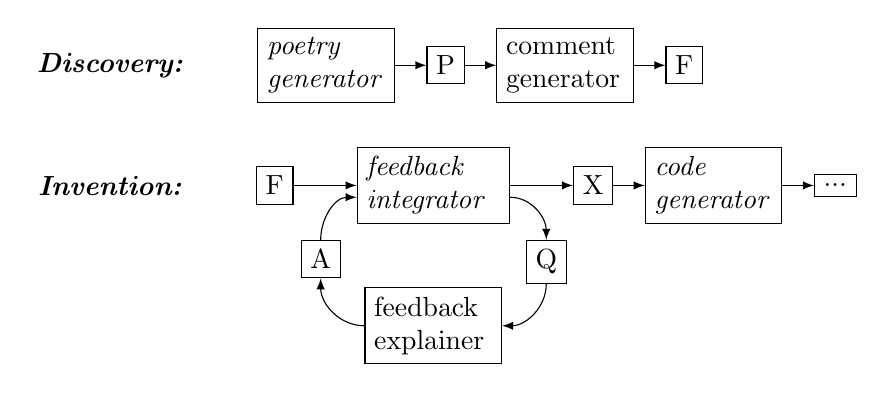
\begin{tikzpicture}[
single/.style={draw, anchor=text, rectangle},
]
\node (discovery) {\textbf{\emph{Discovery:}}};
% poet generates poem
\node[single, right=8mm of discovery.east,text width=1.5cm] (poet) {\emph{poetry generator}};
\node[single, right=4mm of poet.east] (poem) {P};
\draw [-latex] (poet.east) -- (poem.west);
% critic listens to poem and offers feedback
\node[single, right=4mm of poem.east,text width=1.5cm] (critic) {comment generator};
\draw [-latex] (poem.east) -- (critic.west);
\node[single, right=4mm of critic.east] (feedback) {F};
\draw [-latex] (critic.east) -- (feedback.west);

%%% Next phase
\node[below=1cm of discovery] (invention) {\textbf{\emph{Invention:}}};
% poet integrates feedback
\node[single, right=8mm of invention.east] (feedbackcont) {F};
\node[single, right=8mm of feedbackcont.east,text width=1.7cm] (integrator) {\emph{feedback integrator}};
\draw [-latex] (feedbackcont.east) -- (integrator.west);

\node[single, below=8mm of integrator.south,text width=1.5cm] (explainer) {feedback explainer};

\node[single, below right=2mm and 2mm of integrator] (question) {Q};
\node[single, below left=2mm and 2mm of integrator] (answer) {A};

\draw[-latex] ([yshift=-1.5mm]integrator.east) to [out=0,in=90] (question.north) ;
\draw[-latex] (question.south) to [out=270,in=0] (explainer.east) ;
\draw[-latex] (explainer.west) to [out=180,in=270] (answer.south) ;
\draw[-latex] (answer.north) to [out=90,in=180] ([yshift=-1.5mm]integrator.west) ;

\node[single, right=8mm of integrator.east] (problem) {X};

\draw [-latex] (integrator.east) -- (problem.west);

% poet reflects on feedback and updates codebase

\node[single, right=4mm of problem.east,text width=1.5cm] (pgrammer) {\emph{code}\\ \emph{generator}};

\draw [-latex] (problem.east) -- (pgrammer.west);

\node[single, right=4mm of pgrammer.east,text width=.3cm] (etc) {...};

\draw [-latex] (pgrammer.east) -- (etc.west);
\end{tikzpicture}

%\includegraphics[width=.8\textwidth]{schematic}

\par}
\smallskip

\subcaption{A boxes-and-arrows diagram, showing one possible implementation architecture}\label{fig:1c}
\end{minipage}
\bigskip

\caption{Three representations of the elements of serendipity}\label{fig:model}
\end{figure}

Figure \ref{fig:1c} expands this schematic into a sketch of the
components of one possible idealised implementation of a serendipitous
system.  An existing \emph{generative process} is assumed.  This may
be based on observations of the outside world, or it may be a purely
computational process.  In any case, its products are passed on to the
next stage.  After running this data through a feedback loop, certain
aspects of the data are singled out, and marked up as
``interesting.''  Note that this designation need not arise all at
once: rather, it the outcome of a \emph{reflective process}.  In the
implementation envisioned here, this process makes use of two primary
functions: $p_1$, which notices particular aspects of the data, and $p_2$, which
offers reflections about those aspects.  Together, these functions build up a
``feedback object,'' $T^{\star}$, which consists of the original data
and further metadata.  This is passed on to an \emph{experimental
  process}, which has the task of verifying that the data
is indeed interesting, and determining what it may be useful for.
This is again an iterative process, relying on functions $p^{\prime}_1$ and $p^{\prime}_2$, which
build a contextual understanding of the trigger by devising experiments and
assessing their results.  Once implications or applications have been found, a result is
generated, which is passed to a final \emph{evaluation process}, and,
from there, to applications.

The ellipses at the end of the workflow in Figure \ref{fig:1c} are
intended to suggest that applications are open-ended; one
important class of applications will result in changes to one or more
of the system's modules, either by expanding the knowledge base
that it draws on, or adjusting its methods.
This corresponds to Merton's notion of ``extending an existing theory''
\cite{merton1948bearing}.
Note that earlier components of the workflow
cannot, in general, anticipate what the subsequent phases will produce
or achieve.  If the system's next steps could be anticipated, we would
not say that the behaviour was serendipitous, and this global condition pushes back on each of the component modules.  
Serendipity does not adhere to one specific part of the system, but to
its operations as a whole.  

Although Figures  \ref{fig:1b} and  \ref{fig:1c}
treat the case of successful serendipity, as indicated in Figure
 \ref{fig:1a}, each step is fallible, as is the system as a whole.
Thus, for example, a trigger that has been initially tagged as interesting may prove to be fruitless.
Similarly a system that implements all of the steps in Figure \ref{fig:1c}, but that for whatever reason never
achieves results of value cannot be said to have potential for serendipity.
However, a system only produces results of high value would also be
suspect, since it would indicate a tight coupling between trigger
and outcome.  Fallibility is a ``meta-criterion'' that transcends the criteria from Section \ref{sec:by-example}.
Summarising, we propose the following:

%\vspace{.5cm}

\begin{mdframed}
\begin{ndef}\label{def:serendipity}
\emph{(1) Within a system with a prepared mind, a previously uninteresting trigger arises due to circumstances that the system does not control, and is classified as interesting by the system; and,}
\emph{(2) The system uses the trigger and prior preparation, together with relevant computational processing, networking, and experimental techniques, to obtain a novel result that is evaluated favourably by the system or by external sources.}
\end{ndef}
\end{mdframed}

The constituent terms in this definition are purposefully general: for
our purposes it is their relationship that matters.  A trigger, for
example, is not defined in terms of a specific data structure, nor is
a bridge constrained to be drawn from a specific set of reasoning
techniques.  We view such generality as a strength, but it does leave
further work for anyone who aims to apply the definition in practice.
Section \ref{specs-overview} presents further structure that helps to
make that work more routine.



\subsection{Using SPECS to evaluate computational serendipity}\label{specs-overview}

In this section, we use the elements of the conceptual framework
described in Section \ref{sec:by-example} help to flesh out this
definition, to develop quite detailed evaluation criteria.
We adapt the \emph{Standardised Procedure for Evaluating Creative Systems} (SPECS),
a high-level, customisable evaluation strategy that was devised to judge the creativity
of computational systems \cite{jordanous:12}.  

In the three step SPECS process, the evaluator defines the concepts
and behaviours that signal creativity, converts this definition into
clear standards, and then applies them to evaluate the target systems.
%
We follow a slightly modified version of Jordanous's earlier evaluation
guidelines, in that rather than attempt a definition and evaluation of
{\em creativity}, we follow the three steps for \emph{serendipity}.

%\vspace{-.3cm}
\subsubsection*{Step 1: Identify a definition of serendipity that your system should satisfy to be considered serendipitous.}
%~\\
%\vspace{-.1cm}

\noindent We adopt the definition of serendipity from Section
\ref{sec:our-model}.

%\vspace{-.3cm}
\subsubsection*{Step 2: Using Step 1, clearly state what standards you use to evaluate the serendipity of your system.}
%~\\
%\vspace{-.1cm}

\noindent With our definition and other features of the model in mind, we propose the following standards for evaluating serendipity in computational systems. These criteria allow the evaluator to assess the degree of seredipity that is present in a given system's operation.

%% Serendipity relies on a reassessment or reevaluation -- a \emph{focus shift} in which something that was previously uninteresting, of neutral, or even negative value, becomes interesting.

\begin{description}[itemsep=16pt]
\item[{(\textbf{A - Definitional characteristics})}] {The system can
  be said to have a {\textbf{prepared mind}}, consisting of previous
  experiences, background knowledge, a store of unsolved problems,
  skills, expectations, readiness to learn, and (optionally) a current
  focus or goal.  It then processes a {\textbf{trigger}} that is at
  least partially the result of factors outside of its control,
  including randomness or unexpected events.  It classifies this
  trigger as interesting, constituting a {\textbf{focus shift}}.  The
  system then uses reasoning techniques and/or social or otherwise
  externally enacted alternatives to create a {\textbf{bridge}} from
  the trigger to a result.  The {\textbf{result}} is evaluated as
  useful, by the system and/or by an external source.}  The evaluator
  should specify all of these aspects relative to the system under
  consideration at a sufficient degree of precision to show their
  processual interconnection.
%%%%%%%%%%%%%%%%%%%%%%%%%%%%%%%%%%%%%%%%%%%%%%%%%%%%%%%%%%%%%%%%%%%%%
\item[{(\textbf{B - Dimensions})}] {Serendipity, and its various
  dimensions, can be present to a greater or lesser degree.  If the
  criteria above have been met, we consider the system (and
  optionally, generate ratings as estimated probabilities) along
  several dimensions:
%
{($\mathbf{a}$: \textbf{chance})} how likely was this trigger to appear to
  the system?
%
{($\mathbf{b}$: \textbf{curiosity})} On a population basis, comparing
similar circumstances, how likely was the trigger to be identified as
interesting?
%
{($\mathbf{c}$: \textbf{sagacity})} On a population basis, comparing
similar circumstances, how likely was it that the trigger would be
turned into a result?
%
Finally, we ask, again, comparing similar results where possible:
{($\mathbf{d}$: \textbf{value})} How valuable is the result that
is ultimately produced?}
%
%Then combining $\mathbf{a}\times\mathbf{b}\times\mathbf{c}$ gives a
 % likelihood score: 
{Low but nonzero likelihood $\mathbf{a}\times\mathbf{b}\times\mathbf{c}$ 
 and high value $\mathbf{d}$ are the criteria we use to say that the event was ``highly serendipitous.''}
%%%%%%%%%%%%%%%%%%%%%%%%%%%%%%%%%%%%%%%%%%%%%%%%%%%%%%%%%%%%%%%%%%%%%
\item[{(\textbf{C - Factors})}] {Finally, if the criteria from Part A
  are met, and if the event is deemed sufficiently serendipitous to
  warrant further investigation according to the criteria in Part B,
  then in order to deepen our qualitative understanding of the
  serendipitous behaviour, we ask: To what extent does the system
  exist in a {\textbf{dynamic world}}, spanning {\textbf{multiple
      contexts}}, featuring {\textbf{multiple tasks}}, and
  incorporating {\textbf{multiple influences}}?}
\end{description}

%\vspace{-.3cm}
\subsubsection*{Step 3: Test your serendipitous system against the standards stated in Step 2 and report the results.}
%~\\
%\vspace{-.1cm}

\noindent In Section \ref{sec:computational-serendipity}, we will pilot our framework by examining the degree of serendipity of existing and hypothetical computational systems. 

\subsection{Heuristics}\label{specs-heuristics}

How can we we estimate the chance of the trigger appearing, if every
trigger is unique?  Consider de Mestral's encounter with burrs.
The probability of encountering burrs while out walking is high: many
people have had that experience.  The unique features of de Mestral's
experience are that he had the curiosity to investigate the burrs
under a microscope, and the sagacity (and tenacity) to turn what he
discovered into a successful product.  The details of the particular
burrs that were encountered effectively irrelevant.  In the genera case, we are not interested in the chance of encountering a particular object or set of data, which may be vanishingly small.  Rather, we are interested the chance of encountering a trigger that could precipitate an interested response.  The trigger itself may be a complex object or event that takes place over a period of time; in other words, it may be a pattern, rather than a fact.  Noticing that a pattern exists is a key aspect of sagacity.

Although it is in no way required by the SPECS methodology outlined
above, many systems (including all of the examples below) have an
iterative aspect.  This means that a result may serve as a trigger for
further discovery.  In such a case it may be important for further
indeterminacy to be introduced to the system, lest the results be
convergent, and therefor, non-fallible.  In applying the critera to
such systems, we consider long-term behaviour.



\section{Serendipity in computational systems} \label{sec:computational-serendipity}

The 13 facets of serendipity from Section \ref{sec:by-example} specify
the conditions and preconditions that are conducive to serendipitous
discovery.  Section \ref{sec:our-model} distilled these elements into
a computational model.
%
Along with clear criteria, it is important to clearly delineate the
scope of the system being evaluated, and the position of the evaluator
(recalling that ``embedded evaluation'' is a requisite part of a
serendipitous system).  For example, a standard spell-checking program
might suggest a substitution that the user deems especially
fortuitous; and we might agree that serendipity has occurred, but we
would not locate the potential for serendipity in the spell-checker
itself, but rather to the ``cyborg'' system comprised of the user plus
the machine and its software.

\citeA{pease2013discussion} used a simpler variant the SPECS criteria
to analyse three examples of potentially serendipitous behaviour:
dynamic investigation problems, model generation, and poetry
flowcharts.  Using our updated criteria, we discuss two new examples
below, and revisit poetry flowcharts, reporting on recent work and
outlining the next steps.  The three case studies respectively apply
the criteria to \emph{evaluate} an existing system, \emph{design} a
new experiment, and \emph{frame} a ``grand challenge.''  In the first
case study, the system we evaluate turns out not to be particularly
serendipitous according to our criteria.  This helps to show that our
definition is not overly inclusive.  The second example combines
retrospective and prospective positions, as it integrates design and
prototyping.  As Campbell \citeyear{campbell2005serendipity} writes,
``serendipity presupposes a smart mind,'' and each of these examples
suggest potential directions for further work in computational
intelligence.

%% If the system learns an $N$th fact or
%% If applied to a system which could be described as minimally
%% serendipitous at best, and perhaps not at all serendipitous, does our
%% model identify the lack or presence of serendipity?  
%% %% As example, a spellchecker
%% %% program identifies spelling errors in text input and optionally can
%% %% correct spelling automatically. The only situation we can conceive of
%% %% where serendipity could possibly occur is tenuous; perhaps a suggested
%% %% correction may be incorrect, but may lead the user to interpret the
%% %% correction in an unexpected way. In all other aspects that we have
%% %% considered, spellchecker software would be a decidedly unlikely
%% %% candidate for harbouring serendipitous opportunities.  
%% Traditional spellchecker programs could be said to have a
%% \textbf{prepared mind}, in that they are constructed with internal
%% dictionaries with which to check spelling and ways of deciding what a
%% misspelled word might be.  Given our above discussion of how the
%% system might be serendipitous, the \textbf{serendipity trigger} could
%% be seen as the user misspelling a word and the system suggesting
%% alternative possibilities that the user had not previously conceived.
%% However, the \textbf{bridge} from trigger to serendipitous result (if
%% any) would have been built by the user, not by the system.  With
%% adaptive context-aware text completion tools, we can imagine a
%% ``Cyrano de Bergero'' effect in which the machine finds a
%% serendipitous bridge and offers the \textbf{result} to the user.
%% However, the current generation of text completion tools are known
%% more for infelicities than for exceptional wit.

\subsection{Case Study: Evaluation of an existing evolutionary computing system} \label{sec:evomusic}

\subsubsection{System description}

\citeA{jordanous10} reported a computational jazz improvisation system
(later given the name {\sf GAmprovising} \cite{jordanous:12}) that
uses genetic algorithms.  Reevaluating {\sf GAmprovising} can shed
light on the degree to which evolutionary computing can encourage
computational serendipity.

{\sf GAmprovising} uses genetic algorithms to evolve a population of
\emph{Improvisors}. Each Improvisor is able to randomly generate music
based on various parameters such as the range of notes to be used,
preferred notes, rhythmic implications around note lengths and other
musical parameters, see \cite{jordanous10}. These parameters are what
define the Improvisor at any point in the system's evolution.  After a
cycle of evolution, each Improvisor is evaluated using a fitness
function based on Ritchie's \citeyear{ritchie07} formal criteria for
creativity.  This model relies on user-supplied ratings of the novelty
and appropriateness of the music produced by the Improvisor to
calculate 18 metrics that collectively indicate how creative the
system is.  The fittest Improvisors are used to seed a new generation
of Improvisors, through crossover and mutation operations.

\subsubsection{Application of criteria}

The {\sf GAmprovising} system can be said to have a \textbf{prepared
  mind} through its background knowledge of what musical concepts to
embed in the Improvisors and the evolutionary abilities to evolve
Improvisors.  At any given step, the system's \textbf{trigger}
comprises the combination of previous mutation and crossover
operations, and current user input.  To be clear, in the current
version of the system a human evaluator is largely responsible for the
system's \textbf{focus shift}, since the user tells the system which
improvisations are most valuable, metaphorically drawing a circle around some of the generated examples and saying ``more like this, please.''  \citeA{jordanous10} notes that this
``introduces a fitness bottleneck.''  In future versions of the
system, autonomous evaluation could potentially take over for the
human evaluator.  Once the interesting samples have been collected
(from whatever source), a \textbf{bridge} is then built to new results
through the creation of new Improvisors.  The \textbf{results} are the
various musical improvisations produced by the fittest Improvisors (as
well as, perhaps, the parameters that have been considered fittest).

%% The likelihood of serendipitous evolution is greatly enhanced by the
%% use of random mutation and crossover operations within the genetic
%% algorithm, which increase the diversity of the search space covered by
%% the system during evolution.  
The probability of encountering any particular pair of Improvisor and
user evaluation is vanishingly low, given the massive dimensions of
this search space.  However, there will always be some highest-scoring
Improviser, whose parameters will be used to seed the next round.
accordingly, the \textbf{chance} of a trigger appearing to the
system is ``high.''  The uniqueness of the trigger is not particularly
important.  The evolution of Improvisors captures a sense of the
system's \textbf{curiosity} about how to satisfy the musical tastes of
the human user.  The \textbf{sagacity} of the system corresponds to its
methods for enhancing the likelihood that the user will appreciate a
given Improvisor's music (or similar music) over time.  With little
basis for comparison, we can only say that these two dimensions are
``typical.''  The aim of the system is to maximise the \textbf{value}
of the generated results by employing a fitness function.  Indeed,
the system:
\begin{quote}
``{[}W{]}\emph{as able to produce jazz improvisations which slowly
    evolved from what was essentially random noise, to become more
    pleasing and sound more like jazz to the human evaluator's ears}''
  \cite{jordanous10}.
\end{quote}

\subsubsection{Ruling}
The very reliability of the system ultimately bears against its
overall potential for serendipity.  Following Step 2, Part B of the
SPECS procedure, we find a likelihood measure of
$\mathit{high}\times\mathit{moderate}\times\mathit{moderate}$, with
outcomes of moderate value, so that the system as a whole is ``not
very serendipitous.''  Note that evaluating individual threads as
members of the population of all threads would yield more varied
results.  However, in the version of the system under discussion,
individual threads are effectively equivalent regarding the features
of chance, curiosity, and sagacity.  The only thing to distinguish
them from one another is their value.  Referring to the
moderate-at-best likelihood measure, even those threads which maximise
value cannot be regarded as particularly serendipitous.

\subsubsection{Qualitative assessment}

The {\sf GAmprovising} system does operate in \textbf{dynamic world},
assuming that the user's tastes may change.  A more elaborate version
of the system that could cater to multiple users is not yet
implemented, but would be occupied with a considerably more complex
problem, spanning and integrating \textbf{multiple contexts}.  Even
the current version of the performs \textbf{multiple tasks}, but it
uses one global fitness function; it would be more convincing if the
fitness function evolved to match the user's taste.  \textbf{Multiple
  influences} are present but currently only at compile time, in the
design of the fitness function, and at run time with settings for
musical parameters.  Greater dynamism in future versions of the system
would be likely to increase its potential for serendipity.


\subsection{Case Study: Iterative design in automated programming} \label{sec:flowchartassembly}

\subsubsection{System description}

Here we consider the design of a contemporary experiment with the
{\sf FloWr} flowcharting framework \cite{colton-flowcharting}.  
%
{\sf FloWr} is a tool for creating and running computational
flowcharts, built of small modules called ProcessNodes.
%
For day-to-day user, {\sf FloWr} functions as a visual programming
environment.  However, it can also be invoked programmatically, on the
Java Virtual Machine, or with any language using a new web API.  The
goals of {\sf FloWr} are both to be a user friendly tool for
co-creativity, and to be an autonomous \emph{Flowchart Writer}.  Our
experiment targets the latter scenario, assembling available
ProcessNodes into flowcharts automatically.  This can be viewed as a
simple example of automated programming.

In the backend, {\sf FloWr}'s flowcharts are stored as scripts.  These
detail the names of the involved nodes, together with their (input)
parameters and (output) variable settings.  Connections between nodes
are established when one node's input parameter references the output
variable of another node.
%
Inputs and outputs have constraints.  For instance, the {\tt
  WordSenseCategoriser} node has a {\tt stringsToCategorise}
parameter, which needs to be seeded with an ArrayList of strings.  The node produces useful output only when these strings can be parsed as a space-separated list of words.  Similarly, the node's {\tt requiredSense} parameter needs to be seeded with a string that represents one of the 57 British National Corpus Part of Speech tags.  Given constraints of this nature, the first challenge in automated flowchart assembly is to match inputs to outputs correctly, and to make sure that all required inputs are satisfied.

\subsubsection{Application of criteria}

In the initial experimental design, following \citeA{pease2013discussion},
the system's potential \textbf{triggers} result from random, but constrained,
trial and error with flowchart assembly.  Some valid combinations of nodes will
produce results, and some will not.  Due to the dynamically changing
environment (e.g., updates to data sources like Twitter) some
flowcharts that did not produce results earlier may unexpectedly begin
to produce results.
%
The system's \textbf{prepared mind} lies in a distributed knowledge
base provided by the ProcessNodes, which provide metadata that
describe constraints on their inputs and outputs -- and also in the
global history of successful and unsuccessful combinations.
%
The system will not try combinations that it knows cannot produce
results, but it will try novel combinations and may retry earlier
flowchart specimens that have the chance to become viable.  Turning a
collection of nodes for which no known working combination existed
into a working flowchart is an occasion for a \textbf{focus shift}.
What made this particular combination work?  Is there a pattern that
could be exploited in the future?  It may be that no broader pattern
can be found, and the system will simply record the bare fact that the
combination works (and this is the simple starting point from which we
begin).
%
Successful combinations and any further inferences are stored, and
referred to in future runs.  The \textbf{bridge} to a new result is
accordingly found by informed trial and error, building on previous
outcomes.
%
The basic \textbf{result} the system is aiming to achieve is simply to
generate a new combination of nodes that can fit together and that
generates non-empty output.  Reviewing this design, we observed that
subsequent versions of the system may have more detailed evaluation
functions, setting a higher bar for what counts as success.  For
example, a future version of the system could be tuned to search for
flowcharts that generate poetry \cite{corneli2015computational}.

The \textbf{chance} of finding a novel successful flowchart in any
given sample of nodes is fairly low.  Compared to humans users of {\sf
  FloWr}, the search process is exceptionally \textbf{curious}, since
it tries many combinations programmatically.  However, remembering
viable combinations and avoiding combinations that are known not to
work does not require exceptional \textbf{sagacity}.  At least, this will be
so until the system learns more heuristics for flowchart construction, which would
require not only pattern matching but pattern induction.  At the moment, the
system's criterion for attributing \textbf{value} is simply that the combination
of nodes generates non-empty output; an third-party is not likely to judge such
combinations as useful.

\subsubsection{Ruling}

The associated likelihood score is
$\mathit{low}\times\mathit{low}\times\mathit{high}$, which is
relatively favourable.  However, until there is a more discriminating
way to judge value, the attribution of serendipity to any particular
run seems premature.  This motivates a new set of experiments that
seeks to meaningfully judge the value of explanatory heuristics, generated
flowcharts, and texts.  This will both result in and require increased
sagacity on the part of the system.
%%% JAC - add citations to ICCC papers if they have been accepted.

\subsubsection{Qualitative assessment}

The system operates in a \textbf{dynamic world} that is dynamic in two
ways: first, in the straightforward sense that some of the input
sources, like Twitter, are changing; additionally, in the sense that
the system's knowledge of successful and unsuccessful node
combinations changes over time as well.  The current version of the system
does not seem to deal with \textbf{multiple contexts}.  In a future version of the system,
interaction between different heuristically-driven search processes
would be possible, and could lead to more unexpected results.  Along
these lines, as more goals are added, the system could more readily be
seen to have \textbf{multiple tasks}.  For instance, one search
process could look for narrative outlines, and another process could
look for lines or stanzas to fill out that outline.  As for
\textbf{multiple influences}, the population of ProcessNodes will
constrain (and, as more nodes are added, extend) the possible
strategies for assembling flowcharts.  In addition to this localised
knowledge, a pool of heuristics for matching and authoring patterns
would add to the system's sagacity.  Heuristics for evaluating output
are another place where domain-specific knowledge can be brought to
bear.

\subsection{Case Study: Envisioning artificially intelligent recommender systems} \label{sec:nextgenrec}

\subsubsection{System description}

% Stress distinction between serendipity on the system- vs. serendipity on the user's side.
Recommender systems are one of the primary contexts in computing where
serendipity is currently discussed.  In the context of the current
recommender system literature, `serendipity' means suggesting items to
a user that will be likely to introduce new ideas that are unexpected,
but thar are close to what the user is already interested in.  These
systems mostly focus on supporting \emph{discovery} for the user --
but some architectures also seem to take account of \emph{invention}
of new methods for making recommendations, e.g.~by using Bayesian
methods, as surveyed in \citeNP{shengbo-guo-thesis}.  Current
recommendation techniques that aim to stimulate serendipitous
discovery associate less popular items with high unexpectedness
\cite{Herlocker2004,Lu2012}, and use clustering to discover latent
structures in the search space, e.g., partitioning users into clusters
of common interests, or clustering users and domain objects
\cite{Kamahara2005,Onuma2009,Zhang2011}.  But even in the Bayesian
case, the system has limited autonomy.  A case for giving more
autonomy to recommender systems can be made, especially in complex and
rapidly evolving domains where hand-tuning is cost-intensive or
infeasible.  This suggests the need to distinguish serendipity that
the recommender induces for the user from serendipity that user
behaviour induces in the system.

\subsubsection{Application of criteria}

With this challenge in mind, we ask how serendipity could be achieved
within a next-generation recommender system. In terms of our model,
current systems have at least the makings of a \textbf{prepared mind},
comprising both a user- and a domain model, both of which can be
updated dynamically.  User behaviour (e.g.~following certain
recommendations) or changes to the domain (e.g.~adding a new product)
may serve as a potential \textbf{trigger} that could ultimately cause
the system to discover a new way to make recommendations in the
future.  In the current generation of systems that seek to induce
serendipity for the user, the system aims to induce a focus shift by
presenting recommendations that are neither too close, nor too far
away from what user already knows.  Here the flow of information is
the other way around.  Note, however, that it is unexpected pattern of
behaviour in aggregate, rather than a one-off event, that is likely to
provide grounds for the system's \textbf{focus shift}.  A
\textbf{bridge} to a new kind of recommendation could be created by
looking at exceptional patterns as they appear over time.  For
instance, new elements may have been introduced into the domain that
do not cluster well, or a user may suddenly indicate a strong
preference towards an item that does not fit their preference history.
Clusters may appear in the user model that do not have obvious
connections between them.  A new recommendation strategy that
addresses the organisation's goals would be a valuable
\textbf{result}.

The system has only imperfect knowledge of user preferences and
interests.  At least relative to current recommender systems, the
\textbf{chance} of noticing some particular pattern in user behaviour
seems quite low.  The urge to make recommendations specifically for
the purposes of finding out more about users could be described as
\textbf{curiosity}.  Such recommendations may work to the detriment of
user satisfaction -- and business metrics -- over the short term.  In
principle, the system's curiosity could be set as a parameter,
depending on how much coherence is permitted to suffer for the sake of
gaining new knowledge.  Measures of \textbf{sagacity} would relate to
the system's ability to develop useful experiments and draw sensible
inferences from user behaviour.  For example, the system would have to
select the best time to initiate an A/B test.  A significant amount of
programming would have to be invested in order to make this sort of
judgement autonomously, and currently such systems are beyond rare.
The \textbf{value} of recommendation strategies can be measured in
terms of traditional business metrics or other organisational
objectives.

\subsubsection{Ruling}

In this case, we compute a likelihood measure of
$\mathit{low}\times\mathit{variable}\times\mathit{low}$, with outcomes
of potentially high value, so that such a system is ``potentially
highly serendipitous.''  Realising such a system should be understood
as a computational grand challenge.  If such a system was ever
realised, to maintain high value, continued adaptations would be
required.  If there was a population of super-intelligent systems
along the lines envisioned here, the likelihood measures would have to
be rescaled accordingly.

\subsubsection{Qualitative assessment}

Recommender systems have to cope with a \textbf{dynamic world} of changing user preferences and a changing collection of items to recommend.  A dynamic environment which exhibits some degree of regularity represents a precondition for useful A/B testing.  The system's \textbf{multiple contexts} include the user model, the domain model, as well as an evolving model of its own organisation.  A system matching the description here would have \textbf{multiple tasks}: making useful recommendations, generating new experiments to learn about users, and improving its models.  In order to make effective decisions, a system would have to avail itself of \textbf{multiple influences} related to experimental design, psychology, and domain understanding.  Pathways for user feedback that go beyond answers to the question ``Was this recommendation helpful?'' could be one way make the relevant expertise available.


\afterpage{\clearpage}
\begin{table}[p]
{\centering \renewcommand{\arraystretch}{1.5}
\scriptsize
\begin{tabular}{p{1.4in}@{\hspace{.1in}}p{1.4in}@{\hspace{.1in}}p{1.4in}}
\multicolumn{1}{c}{\textbf{{\footnotesize Evolutionary music}}} 
& \multicolumn{1}{c}{\textbf{{\footnotesize Flowchart assembly}}} 
& \multicolumn{1}{c}{\textbf{{\footnotesize Next-gen.~rec.~sys.}}} 
\\[.05in]
\multicolumn{3}{l}{\em {\textbf{Condition}}} \\
\cline{1-3}
\multicolumn{3}{l}{\em Focus shift} \\[-.1cm]
Driven by (currently, human) evaluation of samples
& Find a pattern to explain a successful combination of nodes
& Unexpected behaviour in the aggregate
\\
\cline{1-3}
~\\[-.1cm]
\multicolumn{3}{l}{\em {\textbf{Components}}} \\
\cline{1-3}
\multicolumn{3}{l}{\em Trigger} \\[-.1cm]
% \textbf{Trigger}
Previous evolutionary steps, in combination with user input
& Trial and error in combinatorial search 
& Input from user behaviour
\\
% \cline{1-3}
\multicolumn{3}{l}{\em Prepared mind} \\[-.1cm]
% \textbf{Prepared mind}
Musical knowledge, evolution mechanisms
& Constraints on node inputs and outputs; history of successes and failures
& Through user/domain model\\
% \cline{1-3}
%\textbf{Bridge}
\multicolumn{3}{l}{\em Bridge} \\[-.1cm]
Newly-evolved Improvisors
& Try novel combinations 
& Elements identified outside clusters\\
% \cline{1-3}
%\textbf{Result}
\multicolumn{3}{l}{\em Result} \\[-.1cm]
Music generated by the fittest Improvisors
& Non-empty or more highly qualified output
& Dependent on organisation goals \\ \cline{1-3}
~\\[-.1cm]
%%%%%%%%%%%%%%%%%%%%%%%%%%%%%%%%%%%%%%%%%%%%%%%%%%%%%%%%%%%%%%%%%%%%%%%%%%%%%%%%%%%%%%%%%%%%%%%%%%%%
\multicolumn{3}{l}{\em \textbf{Dimensions}}  \\
\cline{1-3}
%\textbf{Chance}
\multicolumn{3}{l}{\em Chance} \\[-.1cm]
Looking for rare gems in a huge search space
& Changing state of the outside world; random selection of nodes to try 
& Imperfect knowledge of user preferences and behaviour\\
% \cline{1-3}
%\textbf{Curiosity}
\multicolumn{3}{l}{\em Curiosity} \\[-.1cm]
Aiming to have a particular user take note of an Improvisor
& Search for novel combinations 
& Making unusual recommendations\\
% \cline{1-3}
%\textbf{Sagacity}
\multicolumn{3}{l}{\em Sagacity} \\[-.1cm]
Enhance user appreciation of Improvisor over time, using a fitness function
& Don't try things known not to work; consider variations on successful patterns 
& Update recommendation model after user behaviour \\
% \cline{1-3}
%\textbf{Value} &
\multicolumn{3}{l}{\em Value} \\[-.1cm]
Via fitness function (as a proxy measure of creativity)
& Currently ``non-empty results''; more interesting evaluation functions possible 
& Per business metrics/objectives\\
\cline{1-3}
%%%%%%%%%%%%%%%%%%%%%%%%%%%%%%%%%%%%%%%%%%%%%%%%%%%%%%%%%%%%%%%%%%%%%%%%%%%%%%%%%%%%%%%%%%%%%%%%%%%%
~\\[-.1cm]
\multicolumn{3}{l}{\em \textbf{Factors}} \\
\cline{1-3}
%\textbf{Dynamic world}
\multicolumn{3}{l}{\em Dynamic world} \\[-.1cm]
Changes in the user tastes
& Changing data sources and growing domain knowledge 
& As precondition for testing system's influences on user behaviour\\
%\cline{1-3}
%\textbf{Multiple contexts}
\multicolumn{3}{l}{\em Multiple contexts} \\[-.1cm]
Multiple users' opinions would change what the system is curious about and require greater sagacity
& Interaction between different heuristic search processes would increase unexpectedness 
& User model, domain model, model of its own behaviour\\
% \cline{1-3}
%\textbf{Multiple tasks}
\multicolumn{3}{l}{\em Multiple tasks} \\[-.1cm]
Evolve Improvisors, generate music, collect user input, carry out fitness calculations
& Generate new heuristics and new domain artefacts 
& Make recommendations, learn from users, update models\\
% \cline{1-3}
%\textbf{Multiple influences}
\multicolumn{3}{l}{\em Multiple influences} \\[-.1cm]
Through programming of fitness function and musical parameter combinations
& Learning to combine new kinds of ProcessNodes
& Experimental design, psychology, domain understanding\\
\cline{1-3}
\end{tabular}
\par}
\normalsize
\bigskip

\caption{Summary: applying our computational serendipity model to three case studies\label{caseStudies}}
\end{table}

\subsection{Summary}

Table \ref{caseStudies} summarises how the condition, components,
dimensions and factors in our model of serendipity appear in an
evolutionary music system, in hypothetical ``next-generation''
recommender systems, and in our current work on a flowchart-assembly
system.  Each of the case studies shows clear potential for
serendipity.  There are also clear ways in which the measure of
serendipity could be enhanced.

\begin{enumerate}
\item A future version of the evolutionary music system would be more
  convincingly sagacious if it could evaluate works without user
  intervention.  It might also be able to tailor its fitness function
  to the individual user.  More broadly, interaction between the
  system's tasks and more dynamism in its influences would help
  differentiate individual threads or system runs.  Some elements of
  this population might be deemed more serendipitous than others.

\item  The flowchart assembly process would need more stringent, and
  more meaningful, criteria for value before third-party observers
  would be likely to attribute serendipity to the system.  In addition
  to raising challenges for autonomous evaluation (as in the
  evolutionary music system case), this requirement would impose more
  sophisticated constaints on processing in earlier steps, which would
  require the system to be more sagacious.

\item  The next-generation recommender systems we've envisioned need to
  be able to make inferences from aggregate user behaviour.  This
  points to long-term considerations that go beyond the unique
  serendipitous event.  How ``curious'' should these systems be?  One
  obvious criterion is that short-term value should be allowed to
  suffer as long as expected value is still higher.  The symmetry
  between serendipity on the user side, and serendipity on the system
  side might be exploited.  Current systems seek to induce serendipity
  by making use of implicit connections between clusters, resulting in
  an update to the user's conception of the item space.  In current
  recommender systems, the user is given the responsibility to form
  the bridge, even when triggered by the system.  As a preliminary
  step towards building an artificially-intelligent recommender
  system, users might be explicitly given tasks that are designed to
  trigger serendipity on the system-side.
\end{enumerate}


\input{11related}
\section{Discussion and Related Work} \label{sec:discussion}

In Section \ref{sec:computational-serendipity}, we applied our model
to evaluate the serendipity of an evolutionary music improvisation
system, a hypothetical class of next-generation recommender systems,
and a system for assembling flowcharts.  The model has helped to
highlight directions for development that would increase the potential
for serendipity in existing systems, either incrementally or more
transformatively.  Our model outlines a path towards the development
of systems that can observe events that would otherwise not be
observed, take an interest in them, and transform the observations
into artefacts with lasting value.

In this section, we will show how the model allows for more precise
thinking than other existing work touching on this area.  We then
discuss implications from our findings for future research.

%\subsection{Challenges for future research} \label{sec:recommendations}

Viewing the concepts in Section \ref{sec:by-example} through the
practice scenarios we have discussed, we can describe the following
challenges for research in computational serendipity.

\begin{itemize}
\item \textbf{Autonomy}: Our case studies in Section
  \ref{sec:computational-serendipity} highlight the potential value of
  increased autonomy on the system side.
%% The thought experiment in Section
%% \ref{sec:ww} develops a design illustrating the relationship between
%% creativity at the level of artefacts (e.g.~new poems) and
%% creativity at the level of \emph{problem specification} (learning
%% new poetic concepts).
The search for connections that make raw data into ``strategic data''
is an appropriate theme for research in computational intelligence and
machine learning to grapple with.  In the standard cybernetic model,
we control computers, and we also control the computer's operating
context.  There is little room for serendipity if there is nothing
outside of our direct control.  In contrast with the mainstream model,
von Foerster \citeyear[p. 286]{von2003cybernetics} advocated a
second-order cybernetics in which ``the observer who enters the system
shall be allowed to stipulate his own purpose.''  Accordingly, \emph{a
  primary challenge to the serendipitous operation of computers is
  developing computational agents that specify their own problems.}
\end{itemize}

\begin{itemize}
\item \textbf{Learning}: Each of the case studies considered in
  Section \ref{sec:computational-serendipity} is able to learn from
  experience.  As we considered ways to enhance measures of
  serendipity in these examples, we were led to consider computational
  agents that participate meaningfully in ``our world'' rather than in
  a circumscribed microdomain.  \emph{A second challenge is for
    computational agents to learn more and more about the world we
    live in.}
\end{itemize}

\begin{itemize}
\item \textbf{Sociality}: We may be aided in our pursuit of the
  ``smart mind'' required for serendipity by recalling Turing's
  proposal that computers should ``be able to converse with each other
  to sharpen their wits'' \cite{turing-intelligent}.  Turing
  recognised that computers would have to be coached in the direction
  of social learning, but that once they attain that standard they
  will learn much more quickly.  The four supportive factors for
  serendipity described in this paper resemble nothing more than our
  experience of social reality.  \emph{A third challenge is for
    computational agents to interact in a recognisably social way with
    us and with each other, resulting in emergent effects.}
\end{itemize}

\begin{itemize}
\item \textbf{Embedded evaluation}:
  \citeA{stakeholder-groups-bookchapter} outline a general programme
  for computational creativity, and examined perceptions of creativity
  in computational systems found among members of the general public,
  Computational Creativity researchers, and existing creative
  communities.  We should now add a fourth important ``stakeholder''
  group in computational creativity research: computer systems
  themselves.  System designers need to teach their systems how to
  make evaluations in way that is both reasonable and ethical.  This
  condition is exemplified by the preference for a ``non-zero sum''
  criterion for value introduced in Section \ref{sec:by-example}.
  \emph{A fourth challenge is for computational agents to evaluate
    their own creative process and products.}
\end{itemize}


%% A survey of word occurrences from a recent special issue of
%% \emph{Cognitive Computation} on ``Computational Creativity, Intelligence and Autonomy'' \cite{bishop-erden-special-issue} shows that related themes are broadly
%% active in the research community.  Here
%% \emph{italics} indicates that the word stem accounted for 0.1\% of the
%% article or more; added \textbf{\emph{bold}} indicates that it
%% accounted for 1\% or more.\footnote{Articles were converted to text
%%   via {\tt pdftotext -layout}, individual counts found via {\tt tr
%%     \textquotesingle~\textquotesingle~\textquotesingle\textbackslash
%%     n\textquotesingle~< file.txt | grep -c "stem*"}, and total word counts
%%   via {\tt wc -w}.  The corresponding counts for the \emph{current}
%%   paper are 12, \emph{25}, \emph{16}, \emph{44} and 12.7K.}

%% \medskip

%% {\centering \setlength{\tabcolsep}{3pt} \footnotesize
\begin{tabular}{ccccccccccccccc}
paper \#
&1
&2
&3
&4
&5
&6
&7
&8
&9
&10
&11
&12
&13
&14
\\
\cline{2-15}
"autonom.*"
&0
&\textbf{\emph{32}}
&\emph{12}
&\emph{41}
&0
&1
&\emph{31}
&2
&1
&\emph{92}
&11
&2
&5
&\textbf{\emph{22}}
\\
"learn.*"
&6
&2
&2
&\emph{14}
&\emph{9}
&\textbf{\emph{118}}
&\emph{14}
&\emph{18}
&\emph{44}
&\emph{12}
&11
&\emph{42}
&\emph{44}
&2
\\
"social.*"
&0
&0
&\emph{23}
&\emph{25}
&0
&1
&2
&\emph{10}
&\emph{19}
&\emph{19}
&8
&\emph{21}
&13
&2
\\
"evaluat.*"
&0
&1
&\emph{11}
&\emph{20}
&0
&1
&3
&6
&4
&9
&8
&2
&\textbf{\emph{304}}
&0
\\
\cline{2-15}
total(K)
& 8.3  % &8337 (/ 6 8337.0)
& 2.2  % &2221 (/ 32 2221.0)  0.0135074290859973
& 7.5  % &7507  (/ 12 7507.0) 0.0015985080591447982 (/ 23 7507.0) 0.0026641800985746636 (/ 11 7507.0)0.001465299054216065
& 7.4  % &7453 (/ 41 7453.0) 0.004964443848114853 (/ 14 7453.0) 0.0009392191064001073 (/ 16 7453.0) 0.002146786528914531 (/ 19 7453.0) 0.0025493090030860054
& 8.6  % &8675 (/ 9 8675.0)
& 5.8  % & 5816 (/ 89 5816.0) 0.015302613480055021
&10.3 % &10341 (/ 30 10341.0) 0.002901073397156948
& 9.6  % &9632  (/ 18 9632.0) 0.0018687707641196014  (/ 10 9632.0)0.0010382059800664453
&10.8 % &10851 (/ 36 10851.0) 0.0033176665745092617
&11.6 % &11693 (/ 92 11693.0)0.007867955186863935 (/ 12 11693.0)
&14.4 % &14407 (/ 11 14407.0) 0.0007635177344346498
&10.8 % &10840 (/ 31 10840.0) 0.0028597785977859777
&25.3 % &25326 (/ 13  25326.0)  (/ 44  25326.0) 0.0008291873963515755 (/ 304 25326.0) 0.011174287293690278
& 1.6  % &1673 (/ 21 1673.0) 0.012552301255230125
\\
\end{tabular}
}


%% \bigskip

%% Paper 4, Rob Saunders's \citeyear{saunders2012towards} ``Towards
%% Autonomous Creative Systems: A Computational Approach'' was the only
%% contributed paper to emphasise all four of our themes according to the
%% metric above.  Saunders asks: ``What would it mean to produce an
%% autonomous creative system? How might we approach this task? And, how
%% would we know if we had succeeded?''  He argues for an approach ``that
%% models personal motivations, social interactions and the evolution of
%% domains.''  Paper 10, d'Inverno and Luck's \citeyear{d2012creativity}
%% ``Creativity Through Autonomy and Interaction'', also contains a
%% theoretical engagement with these themes, and presents a formalism for
%% multi-agent systems that could usefully be adapted to model
%% serendipitous encounters.  Both papers are particularly concerned with
%% \emph{motivation}, a topic that relates to both the prepared mind and
%% the theme of embedded evaluation.

%% We believe that our clarifications to the multifaceted concept of
%% serendipity will help encourage future computer-aided (and
%% computer-driven) investigations of the above themes and their
%% interrelationships.  Our extension of SPECS to cover serendipity will
%% be useful for evaluating progress.  We discuss some of our related
%% research plans below.

%\subsection{Future Work} \label{sec:futurework} \label{sec:hatching}

In looking for ways to manage and encourage serendipity, we are drawn
to the approach taken by the \emph{design pattern} community
\cite{alexander1999origins}.
%% The essential features of this approach
%% are described below, but we point out straight away that we propose to
%% use design patterns in rather nonstandard fashion.  These adaptations
%% to the typical design pattern methodology are proposed to parallel the
%% four themes outlined above.
%% \begin{itemize}
%% \item[(1)] We want to encode our design patterns directly in runnable
%%   programs, not just give them to programmers as heuristic guidance.
%% \item[(2)] We want the (automated) programmer to generate new design
%%   patterns, not just apply or adapt old ones.
%% \item[(3)] We want our design patterns themselves, working in
%%   combination, to contribute to the discovery of new emergent problems
%%   and patterns, not just capture the solutions to existing known
%%   problems.
%% \item[(4)] We want our design patterns to play an overt role in the
%%   dynamical systems they describe.
%% \end{itemize}
%%
\citeA{meszaros1998pattern} describe the typical scenario for authors of design
patterns: ``You are an experienced practitioner in your
field. You have noticed that you keep using a certain solution to a
commonly occurring problem. You would like to share your experience
with others.''  There are many ways to describe a solution.
Meszaros and Doble remark, ``What sets patterns apart is their
ability to explain the rationale for using the solution (the `why') in
addition to describing the solution (the `how').''  Regarding the
criteria that pattern writers seek to address: ``The most appropriate
solution to a problem in a context is the one that best resolves the
highest priority forces as determined by the particular context.'' 
%
%% Their article describes a number of criteria relevant to writing
%% good design patterns, e.g. \emph{Clear target audience},
%% \emph{Visible forces}, and \emph{Relationship to other patterns}.
%
A good design pattern \emph{describes} the resolution of forces in the
target domain; in the setting we're interested in, creating a new
design pattern also \emph{effects} a resolution of forces directly.
The use case of design pattern development maps into our diagram of
the basic features of serendipity described in Figure \ref{fig:1b}:

\begin{figure}
\begin{center}
\begingroup
\tikzset{
block/.style = {draw, fill=white, rectangle, minimum height=3em, minimum width=3em},
tmp/.style  = {coordinate}, 
sum/.style= {draw, fill=white, circle, node distance=1cm},
input/.style = {coordinate},
output/.style= {coordinate},
pinstyle/.style = {pin edge={to-,thin,black}}
}

\begin{tikzpicture}[auto, node distance=2cm,>=latex']
    \node [sum] (A-sum1) {};
    \node [input, name=pinput, above left=.7cm and .7cm of A-sum1] (A-pinput) {};
    \node [input, name=tinput, left=2.2cm of A-sum1] (A-tinput) {};
    \node [input, name=minput, below left of=A-sum1] (A-minput) {};
    \node [input, name=minput, right of=A-sum1] (A-moutput) {};

    \draw [->] (A-pinput) -- node{{\footnotesize% $p$:
                                   problem}} (A-sum1);
    \draw [->] (A-tinput) -- node{\vphantom{{\footnotesize g}}{\footnotesize% $T$:
                                                                 context~}} (A-sum1);

    \node [sum, right=2.3cm of A-sum1] (B-sum1) {};
    \node [input, name=pinput, above left=.7cm and .7cm of B-sum1] (B-pinput) {};
    \node [input, name=tinput, left of=B-sum1] (B-tinput) {};
    \node [input, name=minput, below left of=B-sum1] (B-minput) {};
    \node [sum, right=2cm of B-sum1] (B-sum2) {};

    \node [input, name=minput, right of=B-sum2] (B-moutput) {};
    \draw [->] (B-pinput) -- node{{\footnotesize% $p^{\prime}$:
        \vphantom{{\footnotesize p}}rationale}} (B-sum1);

    \draw [->] (A-sum1) -- node{\vphantom{{\footnotesize g}}{\footnotesize %$T^{\star}$:
                                                               solution~~}} (B-sum1);

    \draw [->] (B-sum1) -- node{\vphantom{{\footnotesize g}}{\footnotesize % $R$:
                                                               pattern}} (B-sum2);
    \draw [->] (B-sum2) -- node[text width=1.5cm,execute at begin node=\setlength{\baselineskip}{1ex}]{\footnotesize % $|R|>0$:
                                                                                                       \emph{shared\\knowledge}} (B-moutput);
\end{tikzpicture}

\endgroup
\end{center}

\caption{The components of design patterns mapped to our process schematic}
\end{figure}


%\input{12c-future-work-conclusion}

\input{11related}

\subsection{Challenges for future research} \label{sec:recommendations}

Viewing the concepts in Section \ref{sec:by-example} through the
practice scenarios we have discussed, we can describe the following
challenges for research in computational serendipity.

\begin{itemize}
\item \textbf{Autonomy}: Our case studies in Section
  \ref{sec:computational-serendipity} highlight the potential value of
  increased autonomy on the system side.
The search for connections that make raw data into ``strategic data''
is an appropriate theme for research in computational intelligence and
machine learning to grapple with.  In the standard cybernetic model,
we control computers, and we also control the computer's operating
context.  There is little room for serendipity if there is nothing
outside of our direct control.  In contrast to this mainstream model,
von Foerster \citeyear[p. 286]{von2003cybernetics} advocated a
second-order cybernetics in which ``the observer who enters the system
shall be allowed to stipulate his own purpose.''  \emph{A
  primary challenge for the serendipitous operation of computers is
  developing computational agents that specify their own problems.}
\end{itemize}

\begin{itemize}
\item \textbf{Learning}: Each of the case studies considered in
  Section \ref{sec:computational-serendipity} describes a system that
  is able, in one way or another, to learn from experience.  As we
  considered ways to enhance the measure of serendipity in these
  examples, we were led to consider computational agents that
  participate more meaningfully in ``our world'' rather than in a
  circumscribed microdomain.  Knowledge-intensive development work may
  often be unavoidable, but understanding how to foster serendipity is
  important because it points to the potential of systems learning on
  their own.  \emph{A second challenge is for computational agents to
    learn more and more about the world we live in.}
\end{itemize}

\begin{itemize}
\item \textbf{Sociality}: We may be aided in our pursuit of the
  ``smart mind'' required for serendipity by recalling Turing's
  proposal that computers should ``be able to converse with each other
  to sharpen their wits'' \cite{turing-intelligent}.  Turing
  recognised that computers would have to be coached in the direction
  of social learning, but that once they attain that standard they
  will learn much more quickly.  The four supportive factors for
  serendipity described in this paper resemble nothing more than our
  experience of social reality.  For example, our analysis of {\sf
    GAmprovising} suggested that it should interact more with the
  listener and that individual Improvisers should allow
  themselves to be influenced by each other, rather than working in a
  digital silo.  \emph{A third challenge is for computational agents
    to interact in a recognisably social way with us and with each
    other, resulting in emergent effects.}
\end{itemize}

\begin{itemize}
\item \textbf{Embedded evaluation}:
  \citeA{stakeholder-groups-bookchapter} outline a general programme
  for computational creativity, and examine perceptions of
  computational creativity among members of the general public,
  computational creativity researchers, and existing creative
  communities.  We should now add a fourth important ``stakeholder''
  group in computational creativity research: computer systems
  themselves.  System designers need to teach their systems how to
  make evaluations in a way that is both reasonable and ethical.  This
  condition is exemplified by the preference for a ``non-zero sum''
  criterion for value introduced in Section \ref{sec:by-example}.
  Similar judgements apply when the ``product'' is a new process.
  Within a Kantian framework ``an agent's moral maxims are instances
  of universally-quantified propositions which could serve as moral
  laws -- ones holding for any
  agent'' \cite{powers2005deontological}.
  Embedded evaluation is of immediately pragmatic as well as broader philosophical implacations;
  thus, for example, the latest implementation of {\sf GAmprovising} is limited
  because it is ``poor at using reasoned self-evaluation''
  and ``does not generate novel aesthetic measures''  \cite[pp.~189, 288]{jordanous2012evaluating}.
  \emph{A fourth challenge is for computational agents to evaluate
    their own creative process and products.}
\end{itemize}


\subsection{Future Work} \label{sec:futurework} \label{sec:hatching}

In looking for ways to manage and encourage serendipity, we are drawn
to the approach taken by the \emph{design pattern} community
\cite{alexander1999origins}. 
\citeA{meszaros1998pattern} describe the typical scenario for authors of design patterns:

\begin{quote}
\noindent ``You are an experienced practitioner in your field.  You
have noticed that you keep using a certain solution to a commonly
occurring problem.  You would like to share your experience with
others.''
\end{quote}

\begin{figure}[!t]
\vspace{.3cm}
\begin{center}
\begingroup
\tikzset{
block/.style = {draw, fill=white, rectangle, minimum height=3em, minimum width=3em},
tmp/.style  = {coordinate}, 
sum/.style= {draw, fill=white, circle, node distance=1cm},
input/.style = {coordinate},
output/.style= {coordinate},
pinstyle/.style = {pin edge={to-,thin,black}}
}

\begin{tikzpicture}[auto, node distance=2cm,>=latex']
    \node [sum] (A-sum1) {};
    \node [input, name=pinput, above left=.7cm and .7cm of A-sum1] (A-pinput) {};
    \node [input, name=tinput, left=2.2cm of A-sum1] (A-tinput) {};
    \node [input, name=minput, below left of=A-sum1] (A-minput) {};
    \node [input, name=minput, right of=A-sum1] (A-moutput) {};

    \draw [->] (A-pinput) -- node{{\footnotesize% $p$:
                                   problem}} (A-sum1);
    \draw [->] (A-tinput) -- node{\vphantom{{\footnotesize g}}{\footnotesize% $T$:
                                                                 context~}} (A-sum1);

    \node [sum, right=2.3cm of A-sum1] (B-sum1) {};
    \node [input, name=pinput, above left=.7cm and .7cm of B-sum1] (B-pinput) {};
    \node [input, name=tinput, left of=B-sum1] (B-tinput) {};
    \node [input, name=minput, below left of=B-sum1] (B-minput) {};
    \node [sum, right=2cm of B-sum1] (B-sum2) {};

    \node [input, name=minput, right of=B-sum2] (B-moutput) {};
    \draw [->] (B-pinput) -- node{{\footnotesize% $p^{\prime}$:
        \vphantom{{\footnotesize p}}rationale}} (B-sum1);

    \draw [->] (A-sum1) -- node{\vphantom{{\footnotesize g}}{\footnotesize %$T^{\star}$:
                                                               solution~~}} (B-sum1);

    \draw [->] (B-sum1) -- node{\vphantom{{\footnotesize g}}{\footnotesize % $R$:
                                                               pattern}} (B-sum2);
    \draw [->] (B-sum2) -- node[text width=1.5cm,execute at begin node=\setlength{\baselineskip}{1ex}]{\footnotesize % $|R|>0$:
                                                                                                       \emph{shared\\knowledge}} (B-moutput);
\end{tikzpicture}

\endgroup
\end{center}

\vspace{-.3cm}
\caption{The components of design patterns mapped to our process schematic\label{fig:pattern-schematic}}
\vspace{.5cm}
\end{figure}

\begin{figure}[!t]
\setlist[description]{font=\normalfont\itshape}
{\normalsize
\begin{mdframed}
\vspace{2mm}
\textbf{\emph{Successful error}}~
\begin{description}[leftmargin=0\parindent,labelindent=0em,itemsep=2pt]
\item[{Context.}] You run an organisation with different
  divisions and contributors with {\sl varied expertise}.  People routinely
  discover interesting things that no one knows how to {\sl
    turn into a product}.
\item[{Problem.}]  How can you get the most value from this sort of discovery?
\item[{Solution.}] Allow people to work on pet projects, and encourage
  interaction between people in different divisions.  Set aside time
  for in-house seminars.
\item[{Rationale.}] Prototypes can be discussed, even if they are not
  directly marketable.  Following the interests of contributors
  preserves their autonomy.  Contact with different points of view
  brings additional knowledge to bear.
\item[{Resolution.}] 
Open discussion can
  expose flaws at any stage, and can help to guide work in the direction of
  real innovation.  Participants in these conversations
  will learn something, and will help each other maximise the value of
  the discovery.  
\item[{Example.}] Low-tack restickable glue, discovered by a 3M
  engineer in 1968, ultimately proved useful for making
  Post-it\texttrademark\ Notes, which were launched in 1980 after
  several rounds of in-house prototyping.
\end{description}
\vspace{-1mm}
\end{mdframed}
}
\caption{Standard design pattern template applied to van Andel's \em{Successful error}\label{fig:va-pattern-figure}}
\end{figure}

\noindent There are many ways to describe a solution. Meszaros and Doble remark,
\begin{quote}
\noindent ``What sets patterns apart is their ability to explain the
rationale for using the solution (the `why') in addition to describing
the solution (the `how').''
\end{quote}
Regarding the criteria that pattern writers seek to address: 
\begin{quote}
\noindent ``The most appropriate solution to a problem in a context is
the one that best resolves the highest priority forces as determined
by the particular context.''
\end{quote}

%
%% Their article describes a number of criteria relevant to writing
%% good design patterns, e.g. \emph{Clear target audience},
%% \emph{Visible forces}, and \emph{Relationship to other patterns}.
%
Applying the solution achieves this resolution of forces in the
application domain.
The design pattern itself achieves something further: it encapsulates
knowledge in a brief, shareable form.  Tracing the steps involved, we
see that the creation of a new design pattern is always somewhat
serendipitous (Figure \ref{fig:pattern-schematic}; compare Figure
\ref{fig:1b}).

To van Andel's assertion that ``The very moment I can plan or
programme `serendipity' it cannot be called serendipity anymore,'' we
reply that we can certainly describe patterns -- and programs -- with
built-in indeterminacy.  Moreover, we can foster circumstances that
may make unexpected happy outcomes more likely, by developing systems
that increasingly address the challenges outlined in Section
\ref{sec:recommendations}.  Such systems would have a chance of encountering
unexpected stimuli, becoming curious about them, sagaciously pursuing enquiry
together with others, and assessing the value of any outcomes.  
%
Figure \ref{fig:va-pattern-figure} shows one approach to
planning for serendipity, based on rewriting one of van Andel's
serendipity patterns using the standard design pattern template.  In
future work, we intend to build a more complete serendipity pattern
language -- and put it to work within autonomous programming systems.

% Is ``having a stretch goal'' an example of a serendipity pattern?  I think so!




\section{Conclusion} \label{sec:conclusion}

%
We began by surveying ``serendipity'', developing a broad historical
view, and describing several criteria  which we propose
to be computationally salient.  We reviewed related work; like
\citeA{andre2009discovery}, we propose a two-part definition of
serendipity: \emph{discovery} followed by \emph{invention}.
%
Adapting the ``Standardised Procedure for Evaluating Creative
Systems'' (SPECS) model from \citeA{jordanous:12}, we developed a set
of evaluation standards for serendipity.
%
We used this model to analyse serendipity in the context of
evolutionary music improvisation, recommender systems, and flowcharts.
%
We then reflected back over our definition and analyses, and outlined a programme for
serendipitous computing in the pursuit of \emph{autonomy},
\emph{learning}, \emph{sociality}, and \emph{embedded evaluation} that
would tackle the following challenges:
%
\begin{itemize}
\item \emph{A primary challenge to the serendipitous operation of
  computers is developing computational agents that specify their own
  problems.}
\item \emph{A second challenge is for computational agents to learn
  more and more about the world we live in.}
\item \emph{A third challenge is for computational agents to interact
  in a recognisably social way with us and with each other, resulting
  in emergent effects.}
\item \emph{A fourth challenge is for computational agents to evaluate
  their own creative process and products.}
\end{itemize}
%
In the current work, we have limited ourselves to clarifying
conceptual issues surrounding our definition of serendipty, and
examining their design implications.
% 
We indicate several possible further directions for implementation
work in each of our case studies.  We have also drawn attention to
theoretical questions related to program design, with applications to
autonomous programming.  Our examples show that serendipity is not
foreign to computing practice.  There are further gains to be had for
research in computing by planning -- and programming -- for
serendipity.
%



%% \bigskip

%% \noindent \textbf{Acknowledgement.}
%% We appreciate the effort of our anonymous reviewers.


\bibliographystyle{spbasic}
\bibliography{./bibliography/biblio}

% \section{Revision plan}\label{plan-of-action}

\begin{enumerate}
\def\labelenumi{\arabic{enumi}.}
\itemsep1pt\parskip0pt\parsep0pt
\item
  \textbf{(Joe, Alison): Significantly clarify the argument and
  summarise it in the introduction.}
\end{enumerate}

\begin{itemize}
\itemsep1pt\parskip0pt\parsep0pt
\item
  We are offering one possible computational definition of serendipity
\item
  Serendipity is not the same as luck. ~It's a matter of learning
  something, in a way that's unanticipated. ~Looking for something and
  finding something else.
\item
  Explain the aspects of the model better, e.g.~why is it essential that
  the trigger is not under the control of the system.
\item
  Clearly summarise the offering of the paper.
\end{itemize}

\begin{enumerate}
\def\labelenumi{\arabic{enumi}.}
\setcounter{enumi}{1}
\itemsep1pt\parskip0pt\parsep0pt
\item
  \textbf{(Joe): Move our formal definition of serendipity (e.g.~the
  diagram) up to meet the literature review, as a new section `Formal
  definition of Serendipity'. (It's a key contribution of the paper.)}
\end{enumerate}

\begin{itemize}
\itemsep1pt\parskip0pt\parsep0pt
\item
  We will clearly connect the heuristic criteria from Alison with the
  figure.
\item
  In addition a quick graphical summary of the 13 criteria
\end{itemize}

\begin{enumerate}
\def\labelenumi{\arabic{enumi}.}
\setcounter{enumi}{2}
\itemsep1pt\parskip0pt\parsep0pt
\item
  \textbf{(Joe): Drop sections 3 and 4, and move key concepts to
  ``future work''}
\end{enumerate}

\begin{itemize}
\itemsep1pt\parskip0pt\parsep0pt
\item
  Section 3 (FloWr) - heavily condense and put into future work (some
  overview of Joe's concrete implementation plans). ~Explain with
  minimal references.
\item
  Section 4 (Design patterns) - heavily condensed - ``Just So Stories''
  paragraph in Section 5.3 as a potential application. ~Explain some
  history about design patterns and say that, for serendipity, the
  question is where do new ``design'' ideas come from. ~(I.e. discovery
  of a new approach.) ~But make this future work.
\item
  ``We are highlighting how design patterns and the other ideas in this
  paper could be used to build a context where serendipity will take
  place.''
\end{itemize}

\begin{enumerate}
\def\labelenumi{\arabic{enumi}.}
\setcounter{enumi}{3}
\itemsep1pt\parskip0pt\parsep0pt
\item
  \textbf{(Anna): Remove Section 5.3 (save it for another paper about
  Writers Workshops). It's relevant for ``embedded creativity'' but
  ``Writers Workshops'' themselves can be a footnote. The actual idea
  here is more general.}
\end{enumerate}

\begin{itemize}
\itemsep1pt\parskip0pt\parsep0pt
\item
  Anna can add more about evaluation in the creative process
\item
  The idea of the WW (or just social revision) is an example of a place
  where serendipity can occur.
\end{itemize}

\begin{enumerate}
\def\labelenumi{\arabic{enumi}.}
\setcounter{enumi}{4}
\itemsep1pt\parskip0pt\parsep0pt
\item
  \textbf{(Anna): Leading into our thought experiment: ``An emerging
  theme in computing is exploitation of social creativity and feedback.
  Our computational model contributes to theorising this work.''}
\end{enumerate}

\begin{itemize}
\itemsep1pt\parskip0pt\parsep0pt
\item
  Include another example with computational serendipity? Maybe the
  example from Kaz's thesis
\item
  It would not be hard to find an example of a music system noticing
  that a note was wrong and playing. Make sure we include at least one
  example that is not ``technically improbable'' -- better to include
  several that have been realised (e.g.~Copycat)
\end{itemize}

\begin{enumerate}
\def\labelenumi{\arabic{enumi}.}
\setcounter{enumi}{5}
\itemsep1pt\parskip0pt\parsep0pt
\item
  \textbf{(Christian): Copycat or any other historical examples of
  serendipity in computing, or explanation of why there are none (argue
  for or against, in the background section, as a new §§, and perhaps
  again later in the document as a further analysis to accompany our
  thought experiment).}
\end{enumerate}

\begin{itemize}
\itemsep1pt\parskip0pt\parsep0pt
\item
  Concrete lower bound examples and counterexamples, e.g.~would it be
  possible for ``merely generative'' systems to exhibit serendipity? --
  case of genetic algorithms
\item
  What is the difference between serendipity and good luck? (E.g. a
  random act that leads to an outcome that is evaluated positively.)
\item
  What are the strict requirements and what are only the supportive
  factors that make serendipity ``likely''? Or is it a matter of degree?
\item
  Is it the case that serendipitous systems would be more `sagacious' in
  recognizing interesting triggers? - explain, especially in connection
  with computational search.
\item
  What about `regular' systems that work by applying inference
  procedures on symbolic representations to yield new representations?

  \begin{itemize}
  \itemsep1pt\parskip0pt\parsep0pt
  \item
    e.g.~theorem provers
  \end{itemize}
\item
  Evaluate existing approaches to ``computational learning'' - are they
  serendipitous?
\end{itemize}

\begin{enumerate}
\def\labelenumi{\arabic{enumi}.}
\setcounter{enumi}{6}
\itemsep1pt\parskip0pt\parsep0pt
\item
  \textbf{(Simon, Alison): Clarify the extent to which serendipity is
  something that ``actually exists'' or is something that is only
  perceived to exist.}
\end{enumerate}

\begin{itemize}
\itemsep1pt\parskip0pt\parsep0pt
\item
  It does not seem to be an ``essentially contested concept'', just a
  potentially confusing one. One contribution of the paper is to clarify
  this.
\item
  Clarify the relationship to other key concepts in computational
  creativity / creative computing
\end{itemize}

\begin{enumerate}
\def\labelenumi{\arabic{enumi}.}
\setcounter{enumi}{7}
\itemsep1pt\parskip0pt\parsep0pt
\item
  \textbf{(Alison): Include a section early on that defines any other
  keywords that we refer to later, like the word ``dynamic''.}
\item
  \textbf{(Alison): Improve exposition of the analysis of Pek van
  Andel's patterns.}
\end{enumerate}

\begin{itemize}
\item
  \begin{enumerate}
  \def\labelenumi{(\arabic{enumi})}
  \itemsep1pt\parskip0pt\parsep0pt
  \item
    What do we hope to achieve with this analysis, and our diagram?
  \end{enumerate}
\item
  \begin{enumerate}
  \def\labelenumi{(\arabic{enumi})}
  \setcounter{enumi}{1}
  \itemsep1pt\parskip0pt\parsep0pt
  \item
    Have we done the analysis in some verifiable way, i.e. ``where does
    the analysis come from (i.e.~which aspect occurs in which pattern)?
    Is there clear consensus on this?''
  \end{enumerate}
\end{itemize}

\begin{enumerate}
\def\labelenumi{\arabic{enumi}.}
\setcounter{enumi}{9}
\itemsep1pt\parskip0pt\parsep0pt
\item
  \textbf{(Joe, all): Make referencing less intensive for the reader.}
\end{enumerate}

\begin{itemize}
\itemsep1pt\parskip0pt\parsep0pt
\item
  Use APA style referencing and cut down on number of references.
\item
  Clearly explain in narrative form what sort of literature we will draw
  on.
\item
  Perhaps the historical examples of serendipity should be confined to a
  separate ``recommended reading'' section and not referenced directly
  in the text.
\end{itemize}

\begin{enumerate}
\def\labelenumi{\arabic{enumi}.}
\setcounter{enumi}{10}
\itemsep1pt\parskip0pt\parsep0pt
\item
  \textbf{(Christian, Anna): Shorten and improve the literature review.}
\end{enumerate}

\begin{itemize}
\itemsep1pt\parskip0pt\parsep0pt
\item
  Preserve key features of the general survey, but include a more
  thorough review of recent related work in computing, including work in
  the Cognitive Computation journal.
\item
  There has been prior work on surprise (Mary Lou Maher + Kazjon Grace -
  \href{http\%20s://www.google.com/url?q=https\%3A\%2F\%2Fwww.aaai.org\%2Focs\%2Findex.php\%2F\%20WS\%2FAAAIW14\%2Fpaper\%2Fview\%2F8779\&sa=D\&sntz=1\&usg=AFQjCNGFIWctyzoi4ZSfD\%20oIrAznrL4Be0g}{https://www.aaai.org/ocs/index.php/WS/AAAIW14/paper/view/8779}
  and also their paper at ICCC 2013 or 2014) and discovery (Kaz's AAAI
  paper)
\end{itemize}

\begin{enumerate}
\def\labelenumi{\arabic{enumi}.}
\setcounter{enumi}{11}
\itemsep1pt\parskip0pt\parsep0pt
\item
  \textbf{(Joe): Confine philosophy references (e.g.~Bergson, Deleuze)
  to the background section so that it doesn't confuse anyone about what
  we're actually offering in the paper.}
\end{enumerate}

\begin{itemize}
\itemsep1pt\parskip0pt\parsep0pt
\item
  Don't refer to them in the conclusion, but do summarise the
  contribution of this paper again in the conclusion (hint: it should be
  what we say in the title).
\item
  Re-summarise again in the abstract.
\end{itemize}


\end{document}
